\documentclass[letter,12pt]{article}
\usepackage[letterpaper,right=1in,left=1in,top=1in,bottom=1in]{geometry}
\usepackage[longnamesfirst, sort]{natbib}\bibpunct[]{(}{)}{;}{a}{}{,}
\usepackage{ae} % or {zefonts}
\usepackage[T1]{fontenc}
\usepackage[ansinew]{inputenc}
\usepackage{amsmath}
\usepackage{amssymb}
\usepackage{url}
\usepackage{lscape} %landcape pages support
\usepackage{setspace} %allows to change linespacing
\setstretch{2} %linespacing
%\onehalfspacing
%\doublespacing
\usepackage{pifont} %para tener la ballot cross \ding{55}


\usepackage{tabulary} %calcula autom�ticamente ancho de columnas con texto muy largo
%% usar LRJC para c�lculo autom�tico, lrjc para ancho de columna normal
\setlength\tymin{10pt}       %% estos permiten cambiar conducta, ver p. 254 LaTeX companion
\setlength\tymax{\maxdimen}

\usepackage[pdftex]{graphicx}
%\usepackage{graphicx}
\graphicspath{"c:/data"}
\usepackage{color}
%\usepackage[colorlinks]{hyperref}
\usepackage{tikz} % Easier syntax to draw pgf files (invokes pgf automatically)
\usetikzlibrary{arrows,shapes.geometric}
%\usepackage{pgfmath}

\usepackage{rotating}% allows sideways tables or other stuff

% to change margins in a section -- type \begin{changemargin}{deltaLEFT}{deltaRIGHT}
\def\changemargin#1#2{\list{}{\rightmargin#2\leftmargin#1}\item[]}
\let\endchangemargin=\endlist

\begin{document}

\setstretch{1} %linespacing

\textbf{Trabajo final de Elecci�n P�blica III --- la entrega ser� a las 12h00 del lunes 23 de mayo de 2011 en mi oficina.}

\bigskip

Seg�n Cox y McCubbins (2005), aunque es com�n que el partido legislativo mayoritario, como cualquier partido, manifieste divisiones en sus filas, \emph{nunca} debiera de dividirse en el pleno. Esto es, gracias al control de la agenda, nunca deben observarse confrontaciones entre las facciones del partido mayoritario en votaciones nominales. Explique la parad�jica divisi�n del PRD en la ALDF entre 2006 y 2009.

Cada gr�fica presenta la l�nea de corte (\emph{cutline}) de una votaci�n nominal no un�nime en el periodo. Se indica la fecha y votos a favor, en contra, y abstenciones registrados en el pleno. Consulten la fecha espec�fica del diario de sesiones de la ALDF para ver el contenido de la legislaci�n y c�mo votaron los legisladores. Tenga en cuenta que para la estimaci�n us� un modelo de utilidad aleatoria --- dicho de otro modo, hay errores de predicci�n, y algunos cutlines se salen de rango.


\begin{center}
\begin{tabular}{ccccc}
   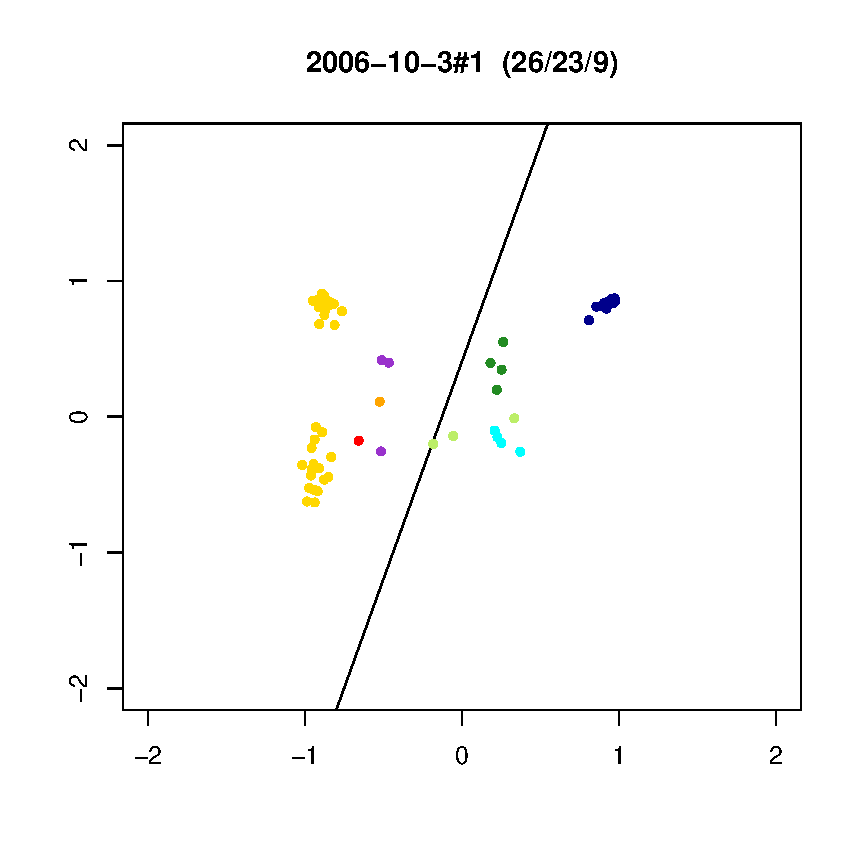
\includegraphics[width=4cm]{cutline1.pdf} &
   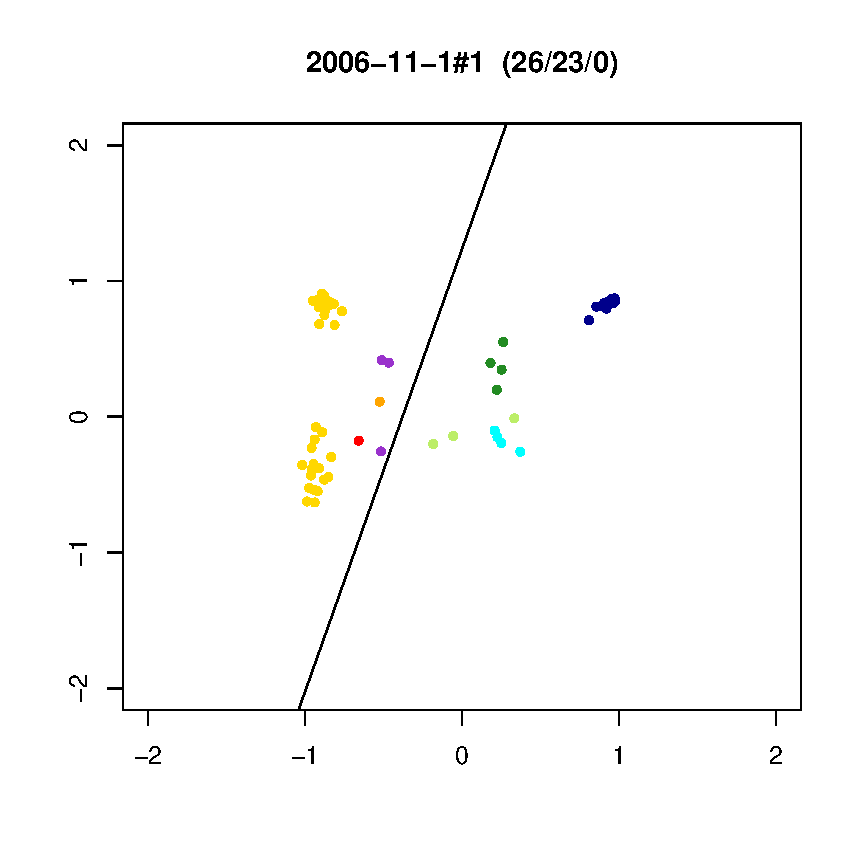
\includegraphics[width=4cm]{cutline2.pdf} &
   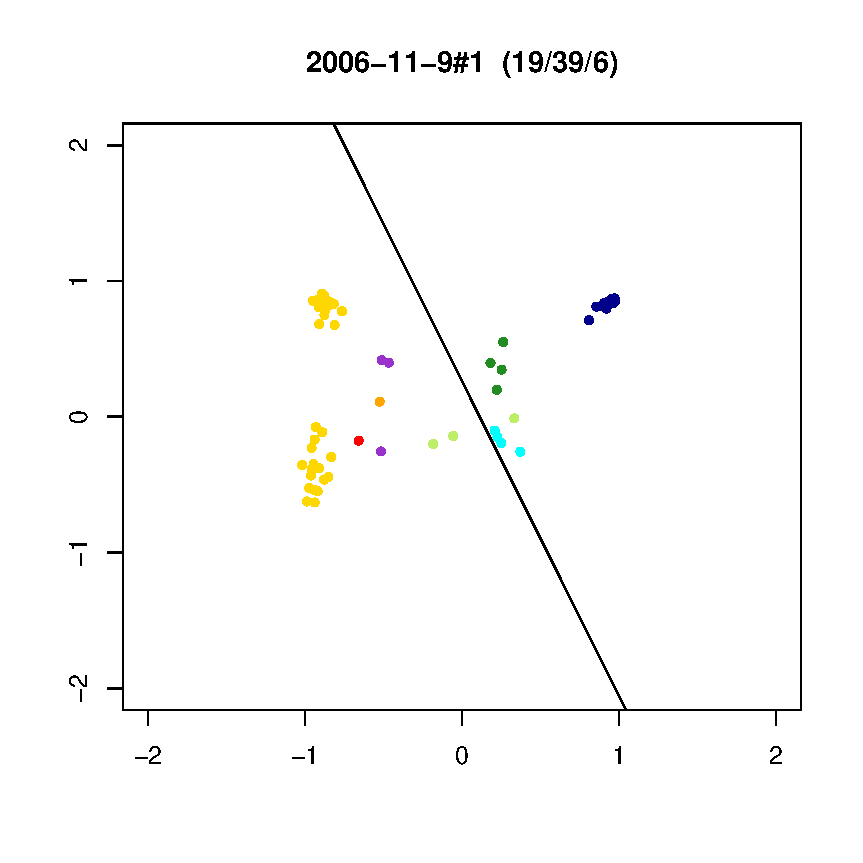
\includegraphics[width=4cm]{cutline3.pdf} &
   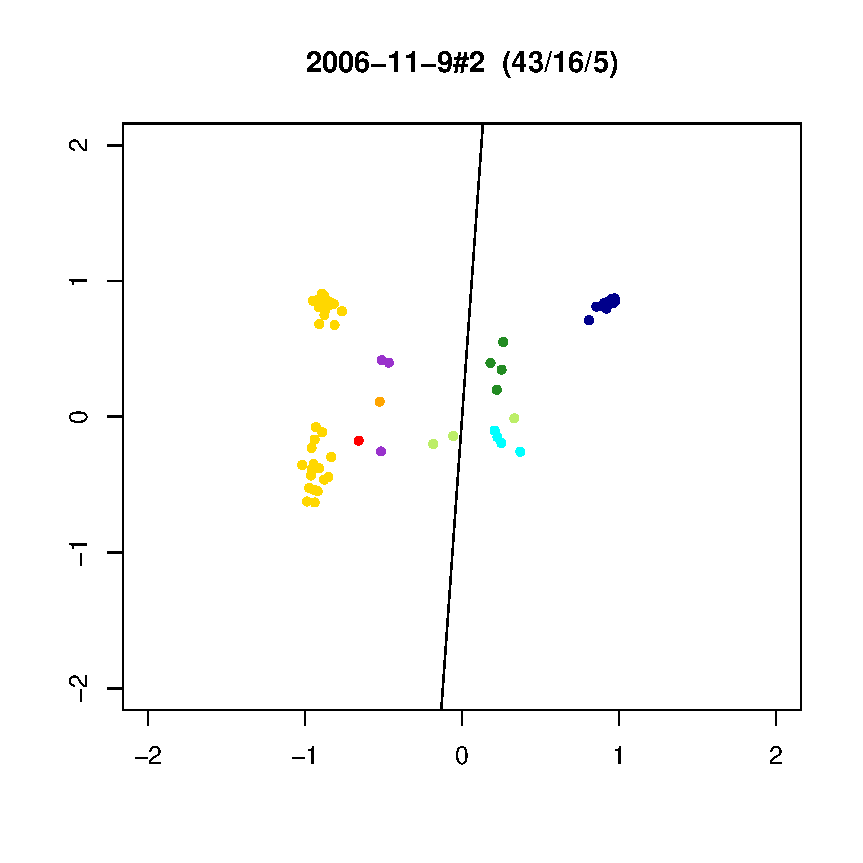
\includegraphics[width=4cm]{cutline4.pdf} \\
   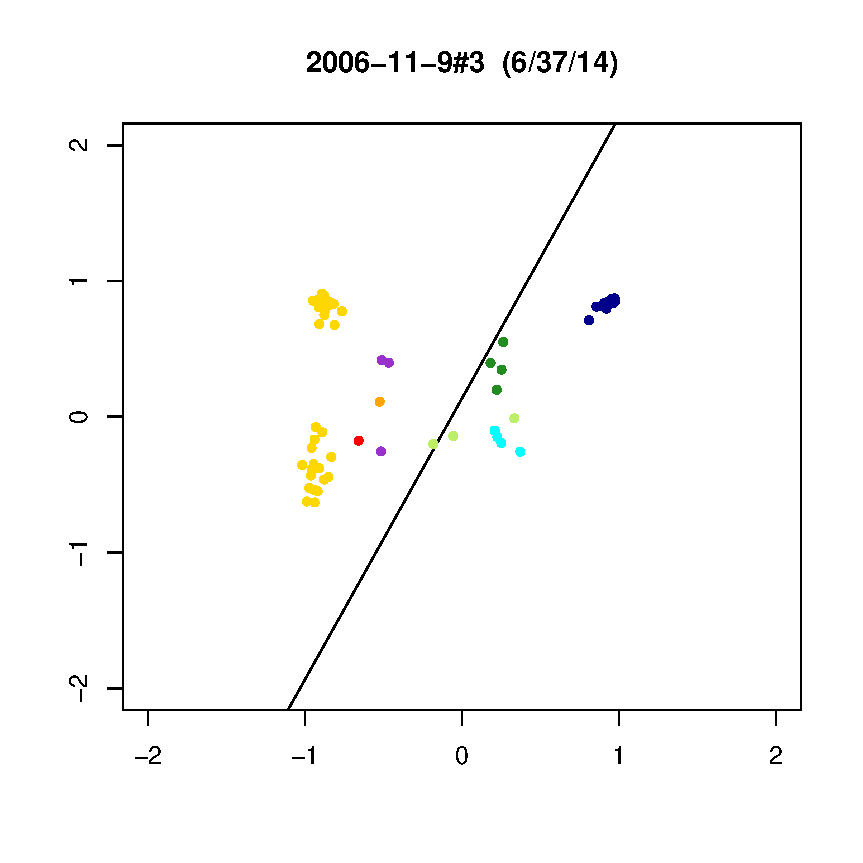
\includegraphics[width=4cm]{cutline5.pdf} &
   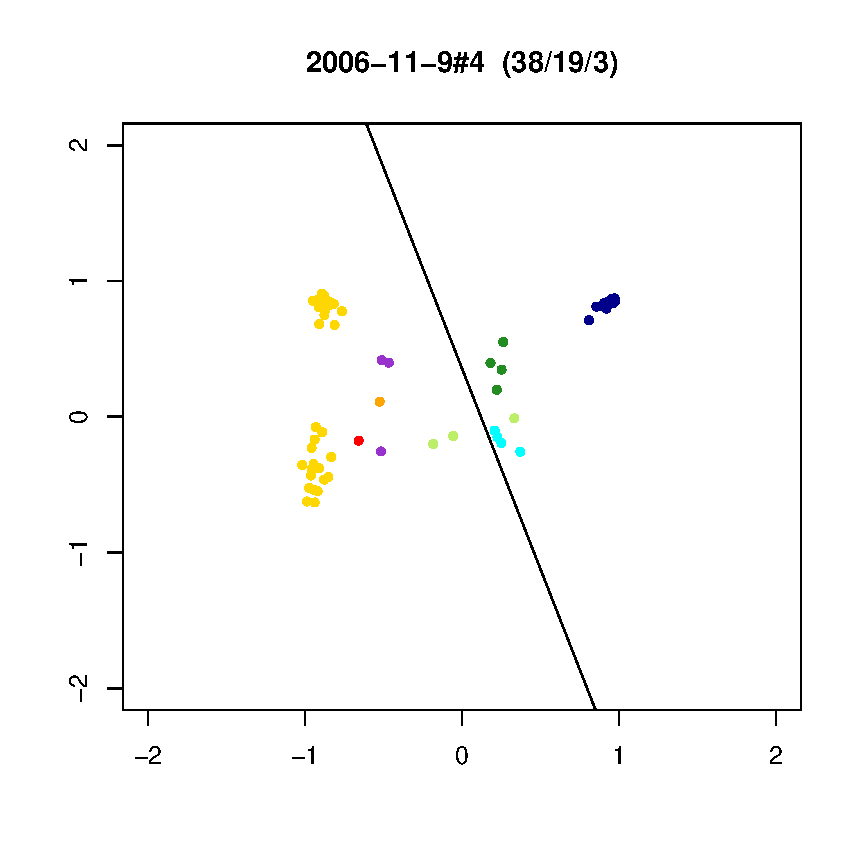
\includegraphics[width=4cm]{cutline6.pdf} &
   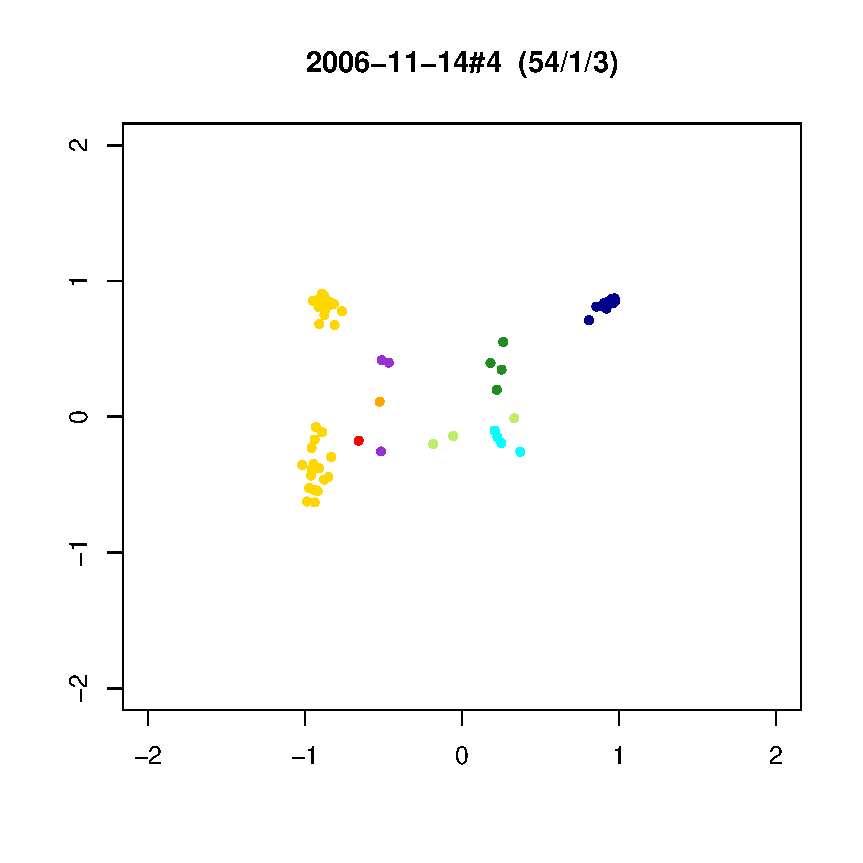
\includegraphics[width=4cm]{cutline7.pdf} &
   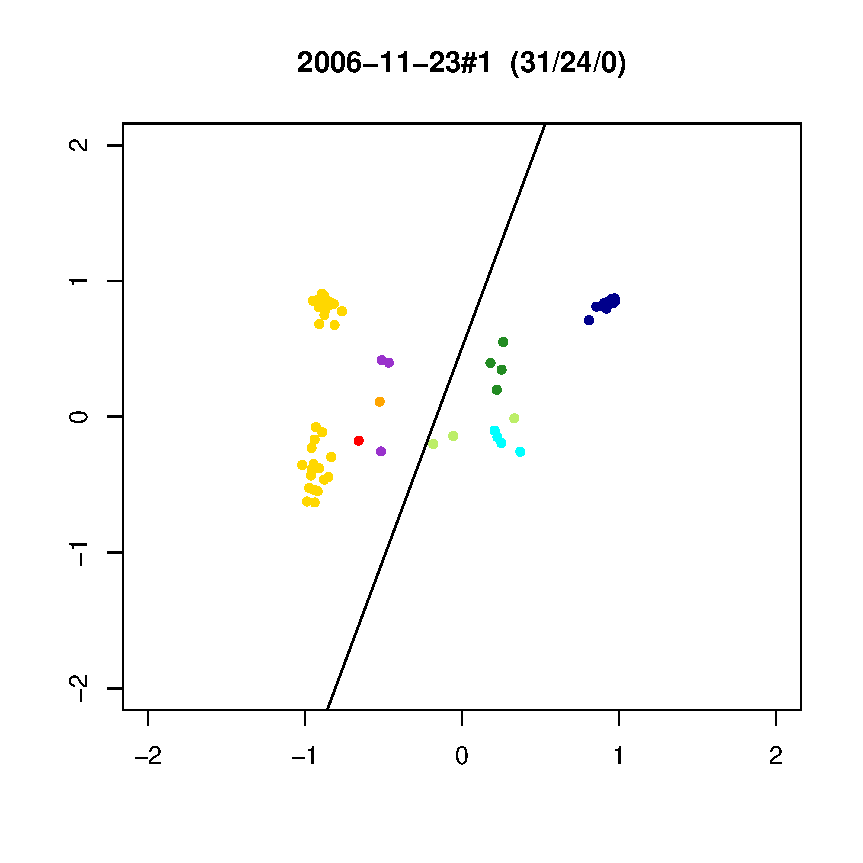
\includegraphics[width=4cm]{cutline8.pdf} \\
   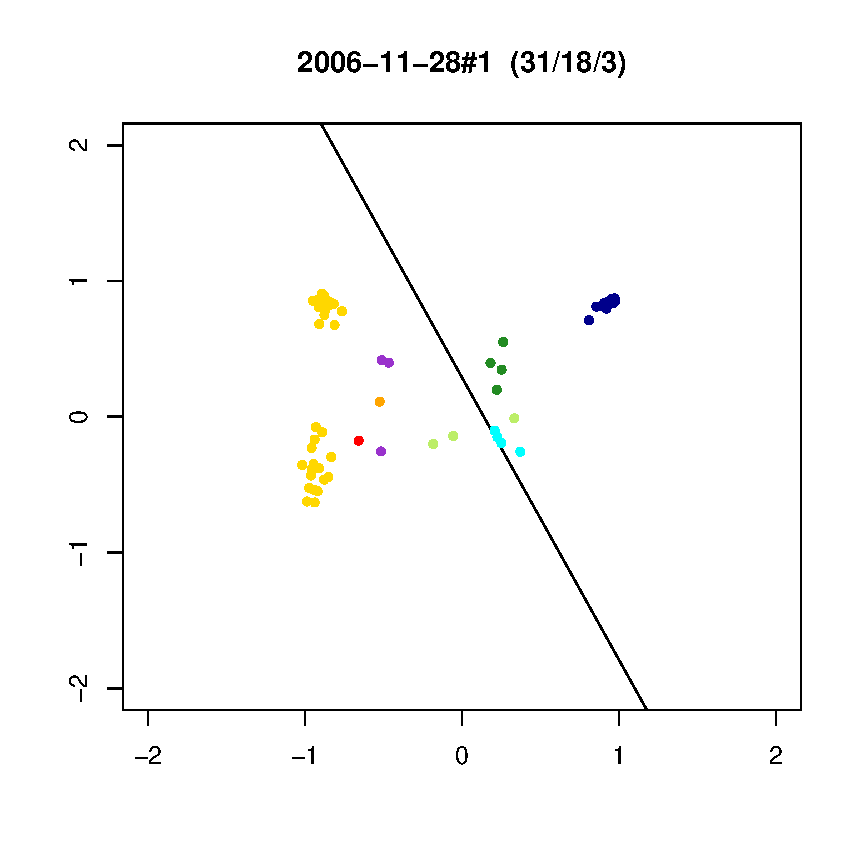
\includegraphics[width=4cm]{cutline9.pdf} &
   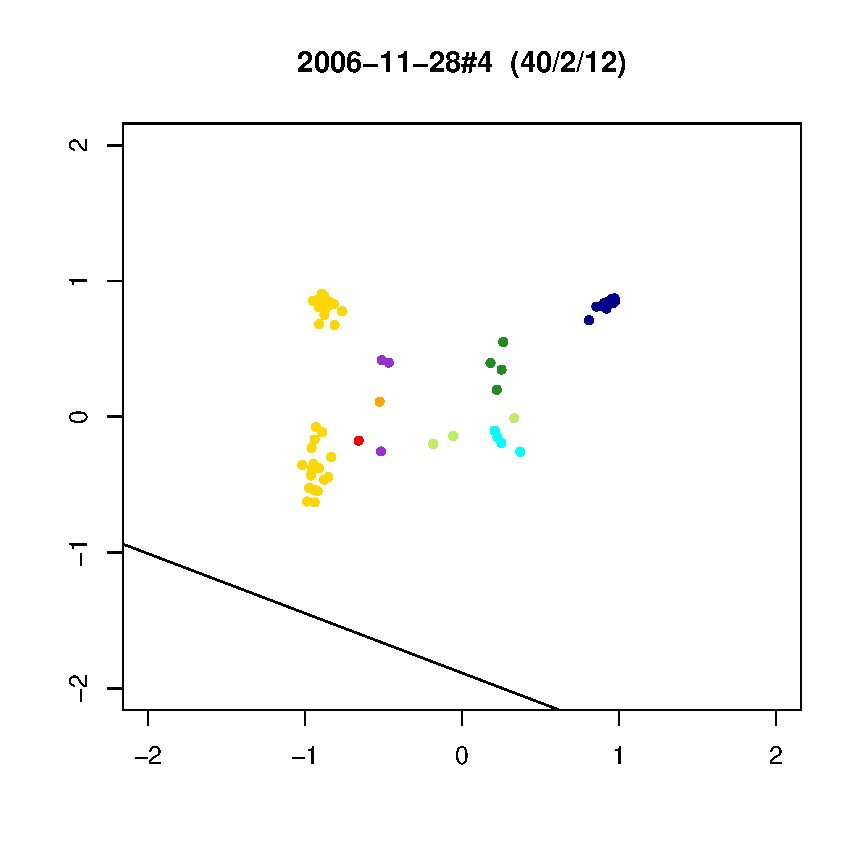
\includegraphics[width=4cm]{cutline10.pdf} &
   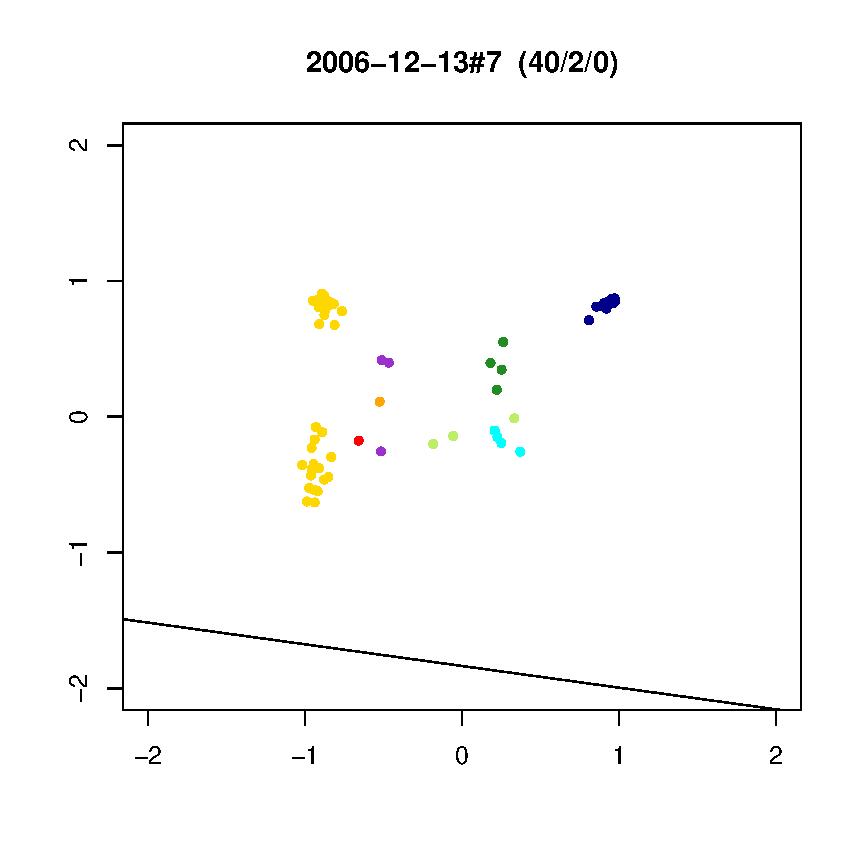
\includegraphics[width=4cm]{cutline11.pdf} &
   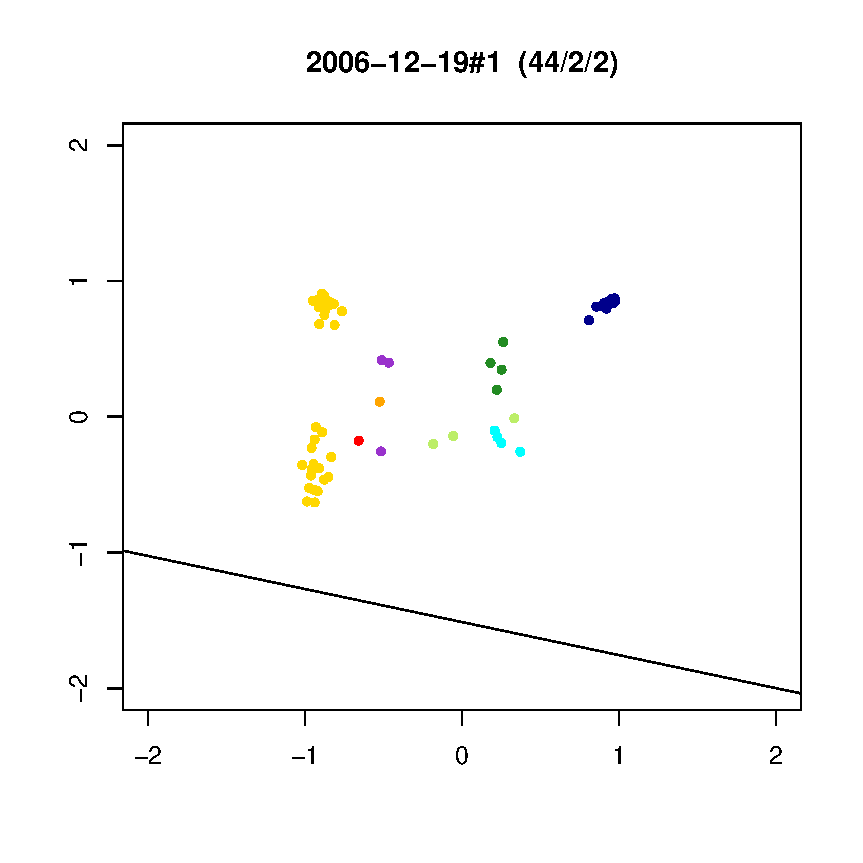
\includegraphics[width=4cm]{cutline12.pdf} \\
   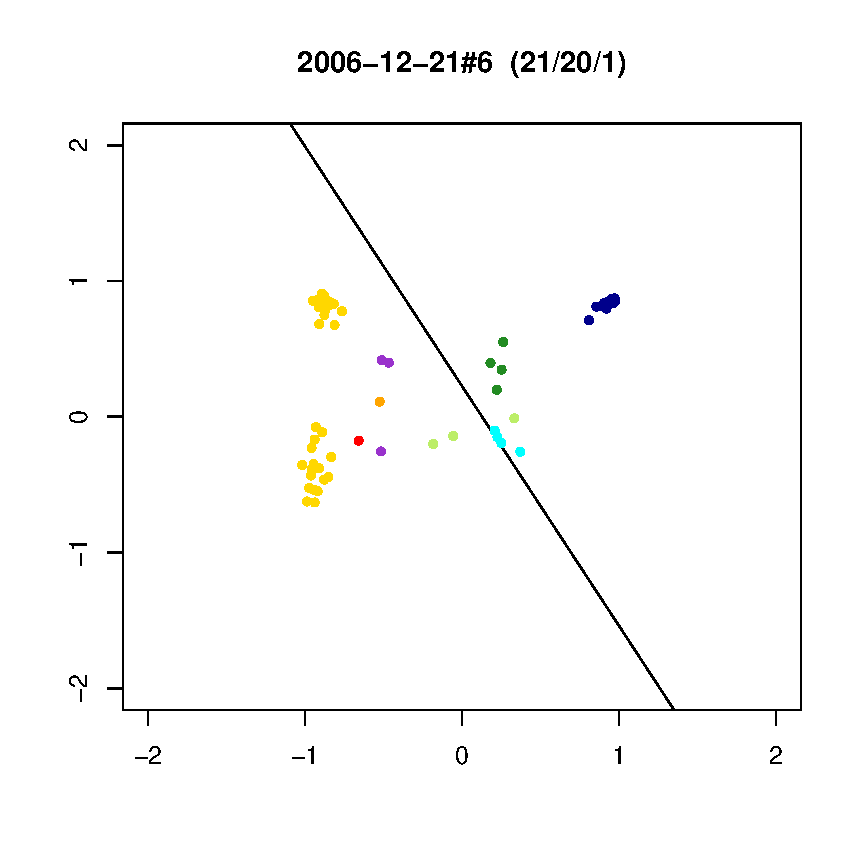
\includegraphics[width=4cm]{cutline13.pdf} &
   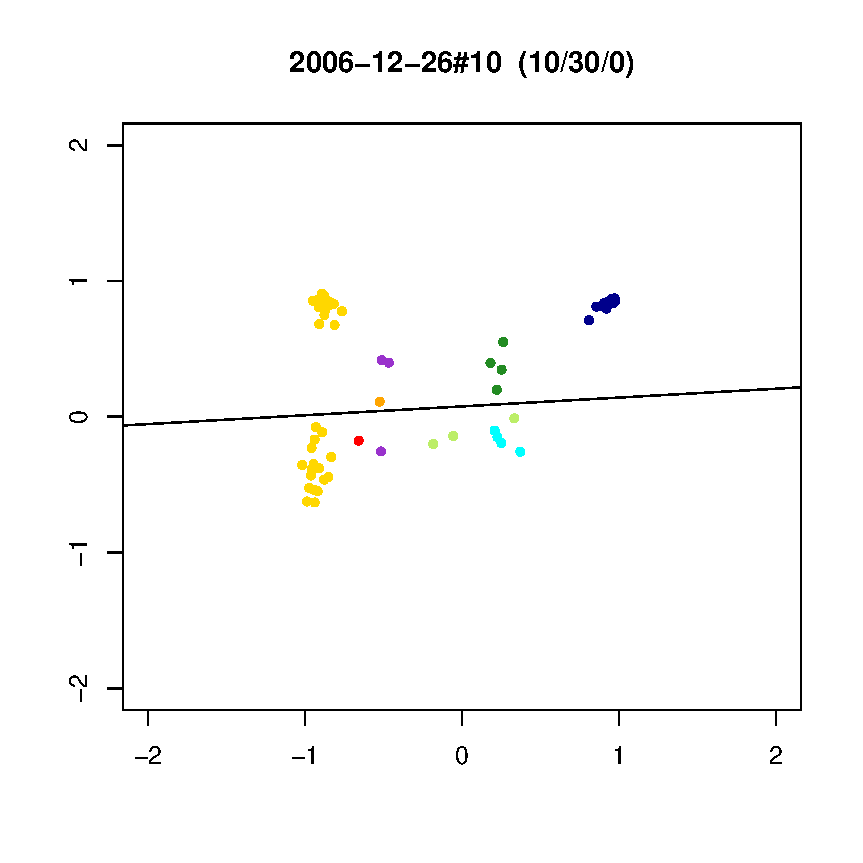
\includegraphics[width=4cm]{cutline14.pdf} &
   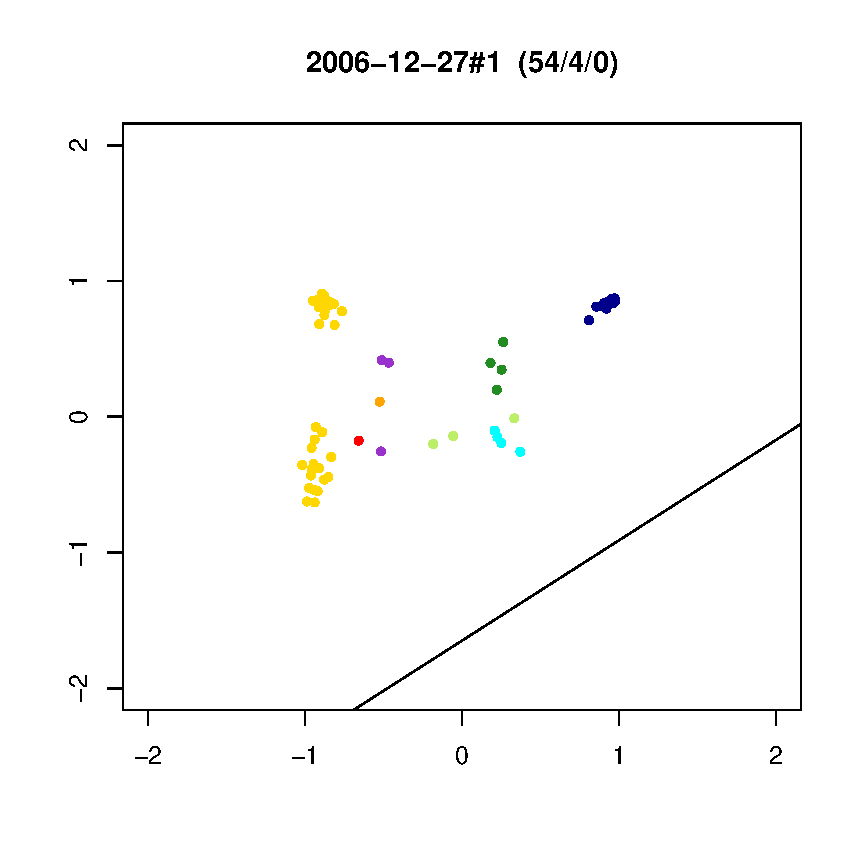
\includegraphics[width=4cm]{cutline15.pdf} &
   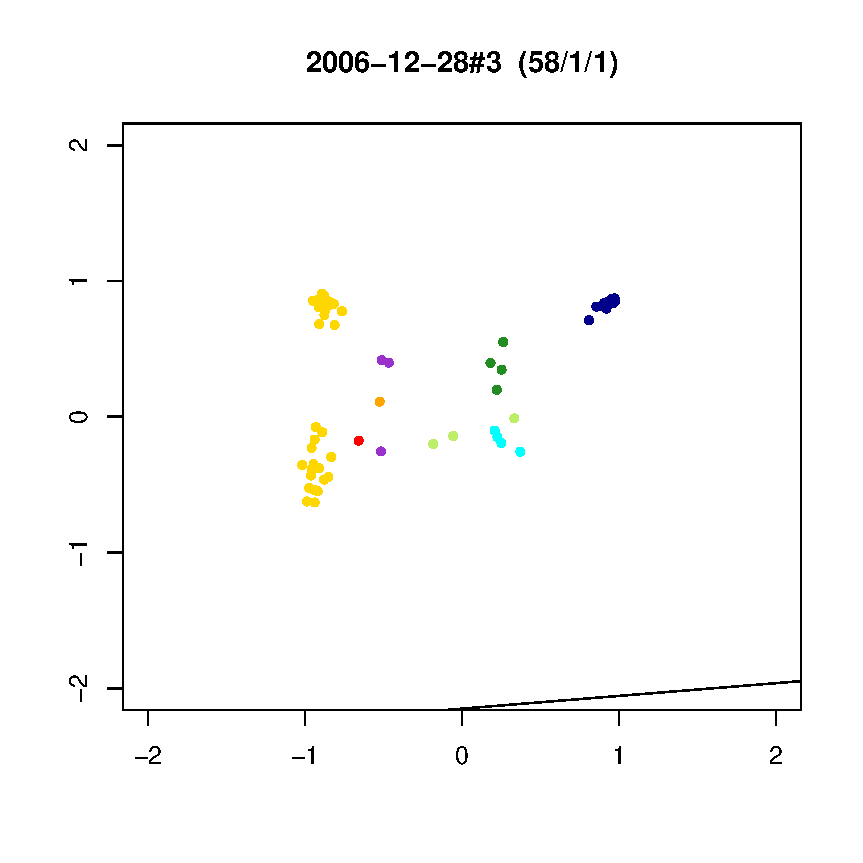
\includegraphics[width=4cm]{cutline16.pdf} \\
   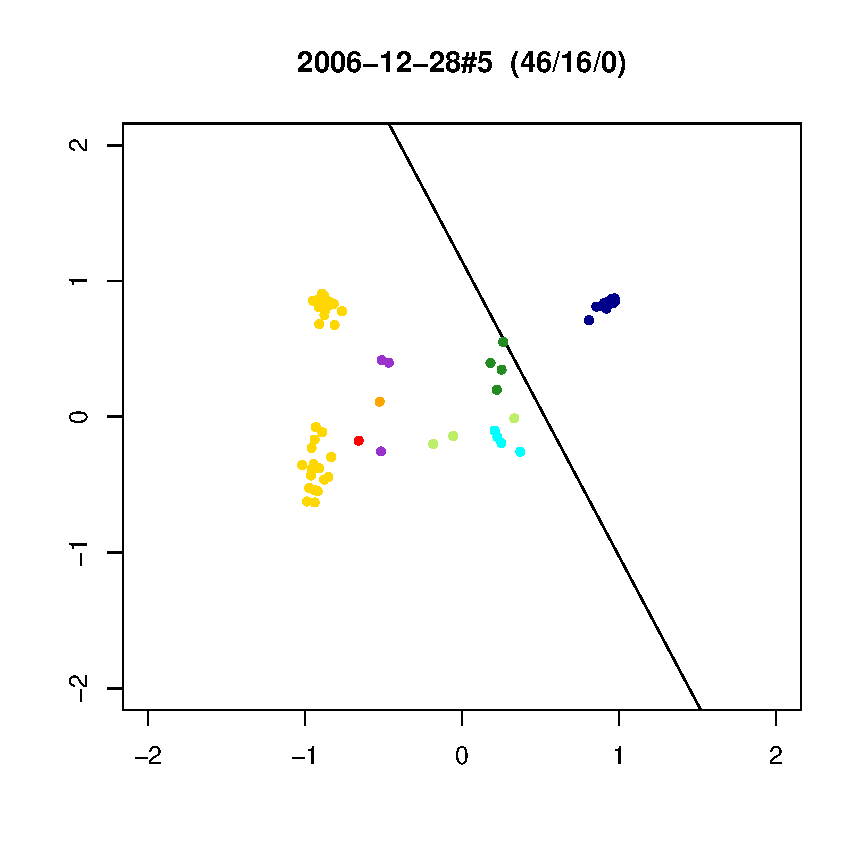
\includegraphics[width=4cm]{cutline17.pdf} &
   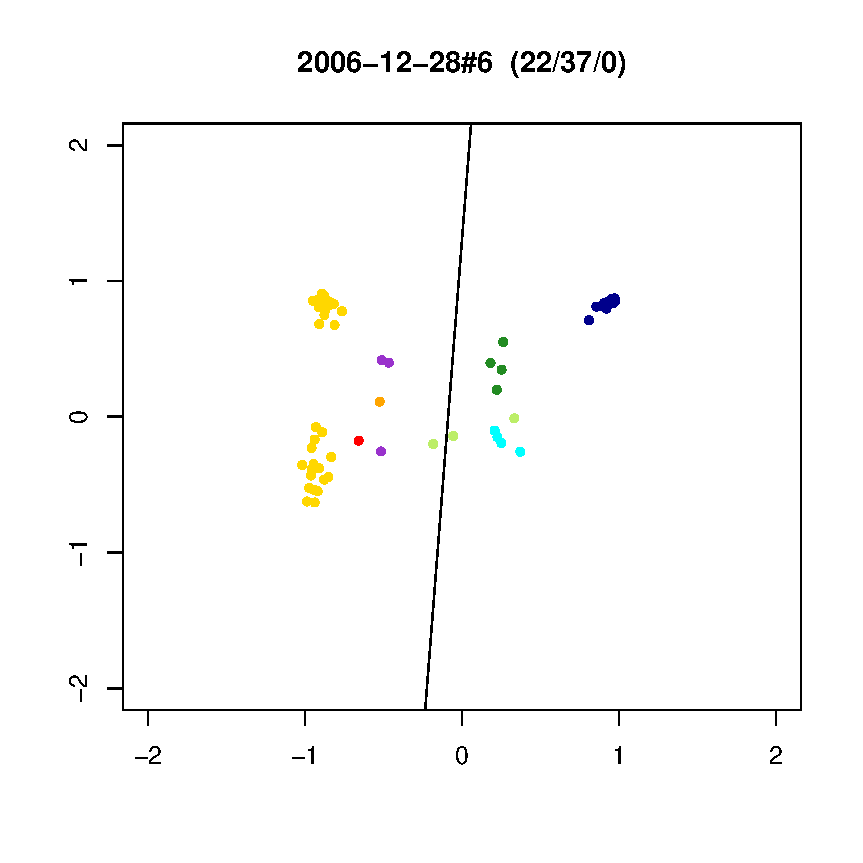
\includegraphics[width=4cm]{cutline18.pdf} &
   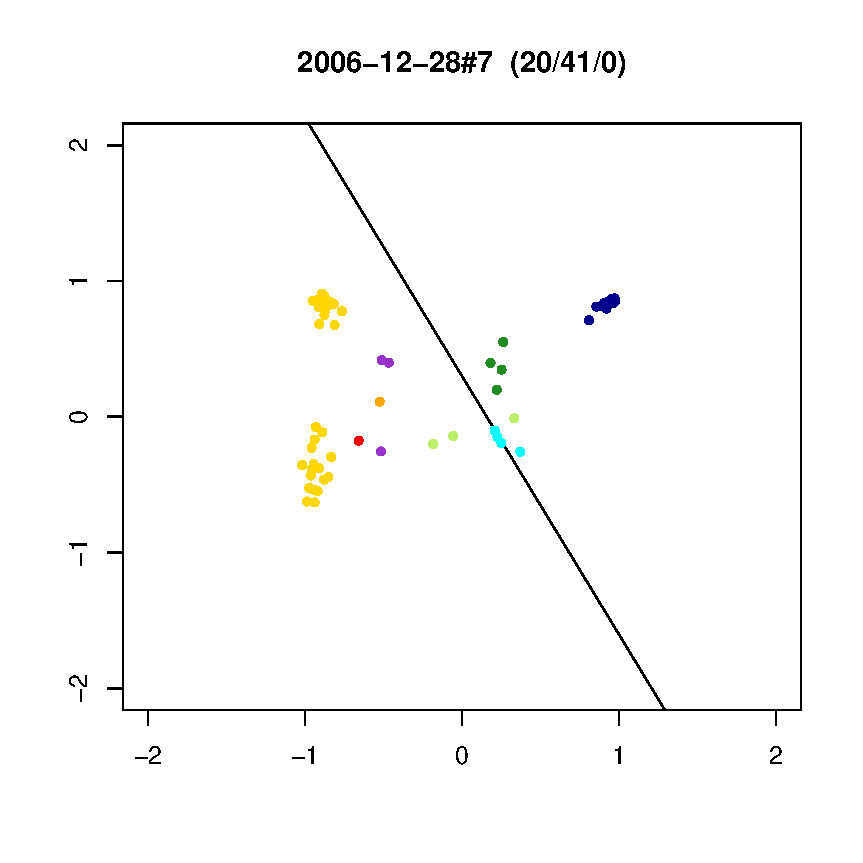
\includegraphics[width=4cm]{cutline19.pdf} &
   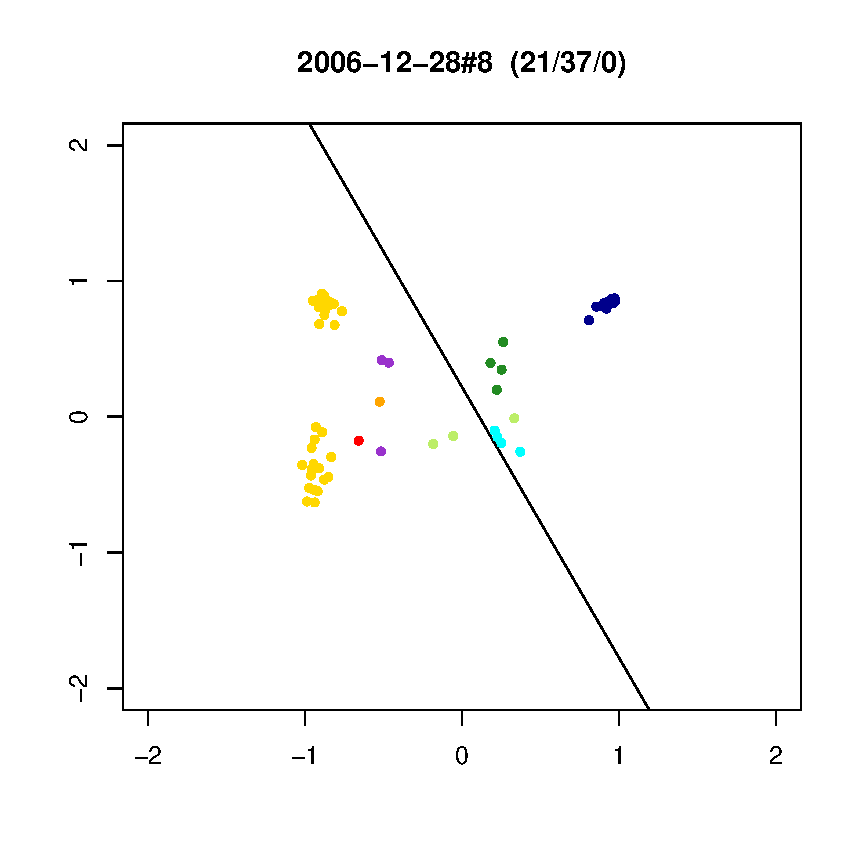
\includegraphics[width=4cm]{cutline20.pdf} \\
\end{tabular}
\end{center}

\newpage

\begin{center}
\begin{tabular}{ccccc}
   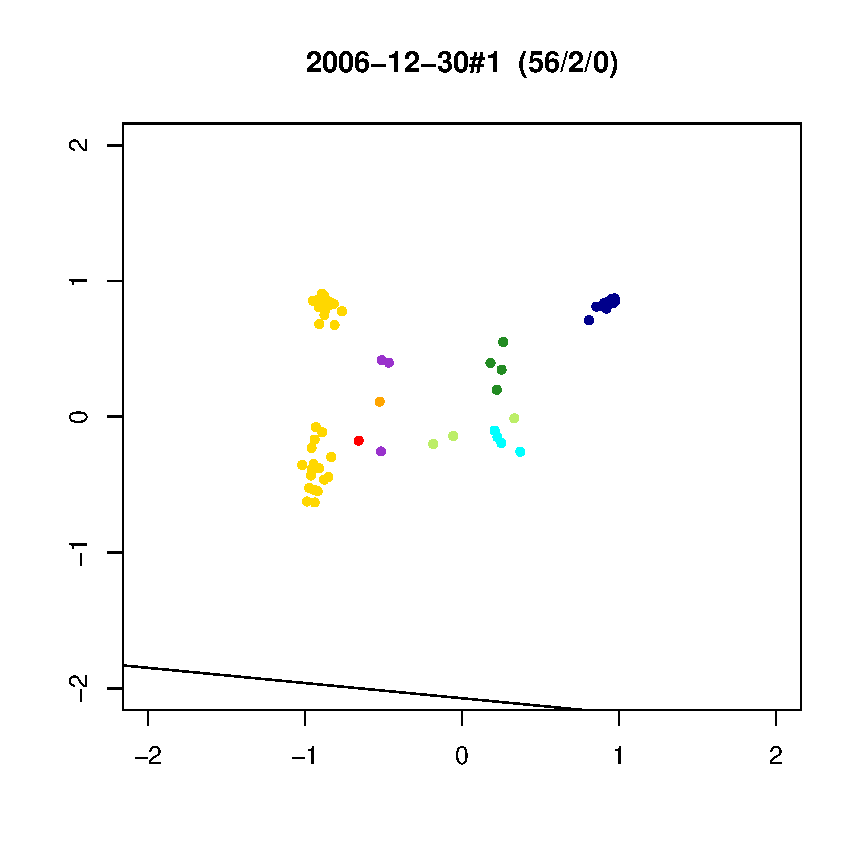
\includegraphics[width=4cm]{cutline21.pdf} &
   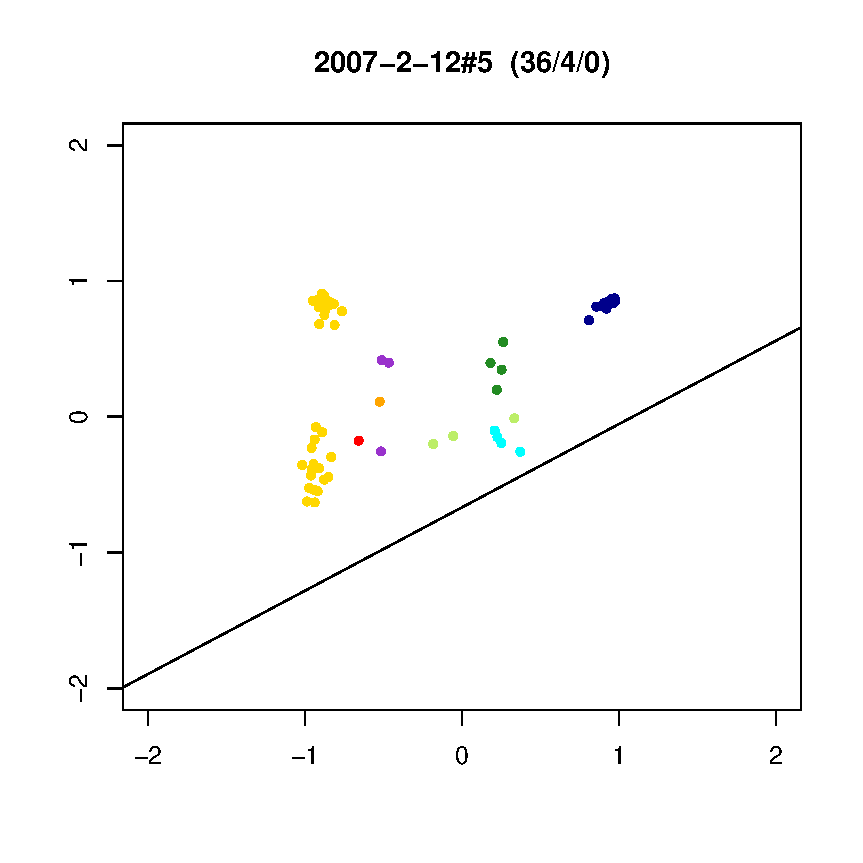
\includegraphics[width=4cm]{cutline22.pdf} &
   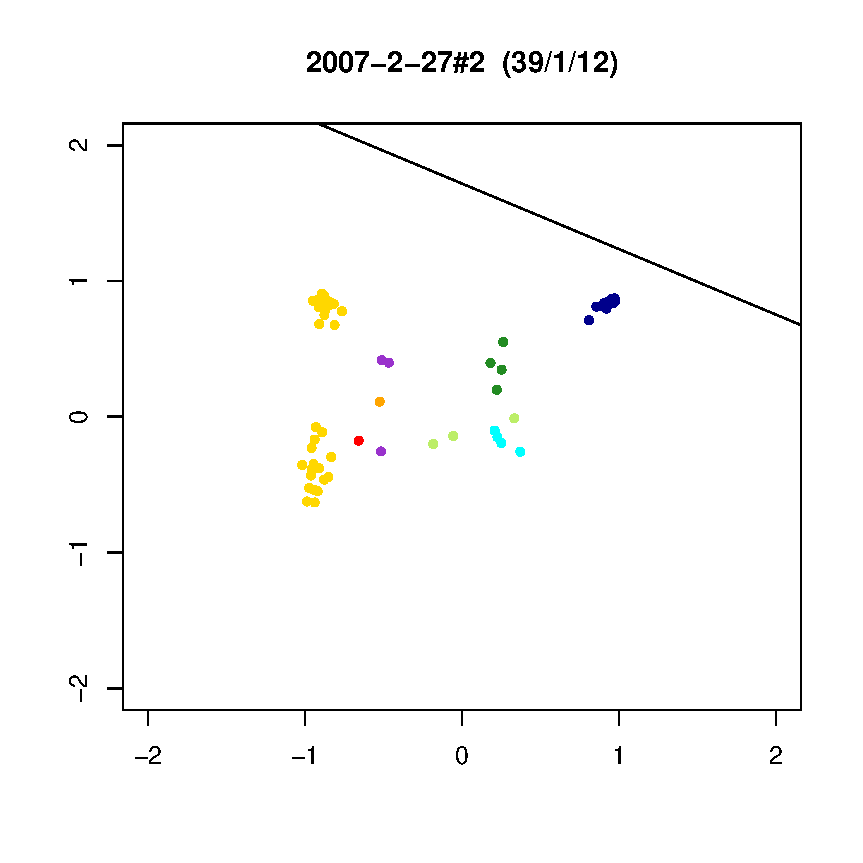
\includegraphics[width=4cm]{cutline23.pdf} &
   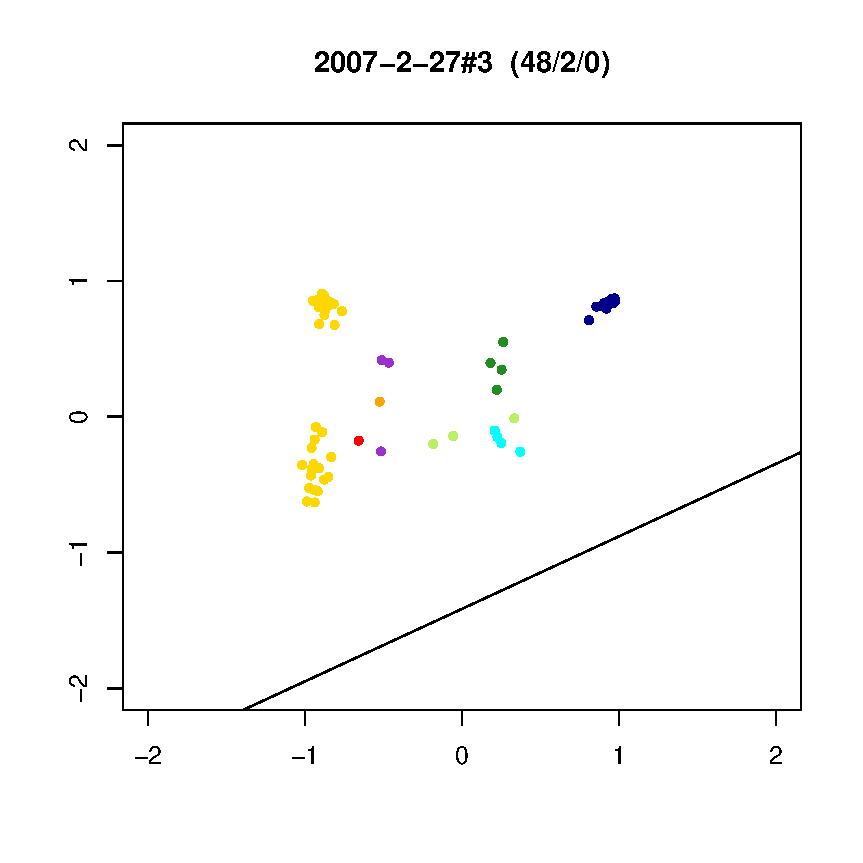
\includegraphics[width=4cm]{cutline24.pdf} \\
   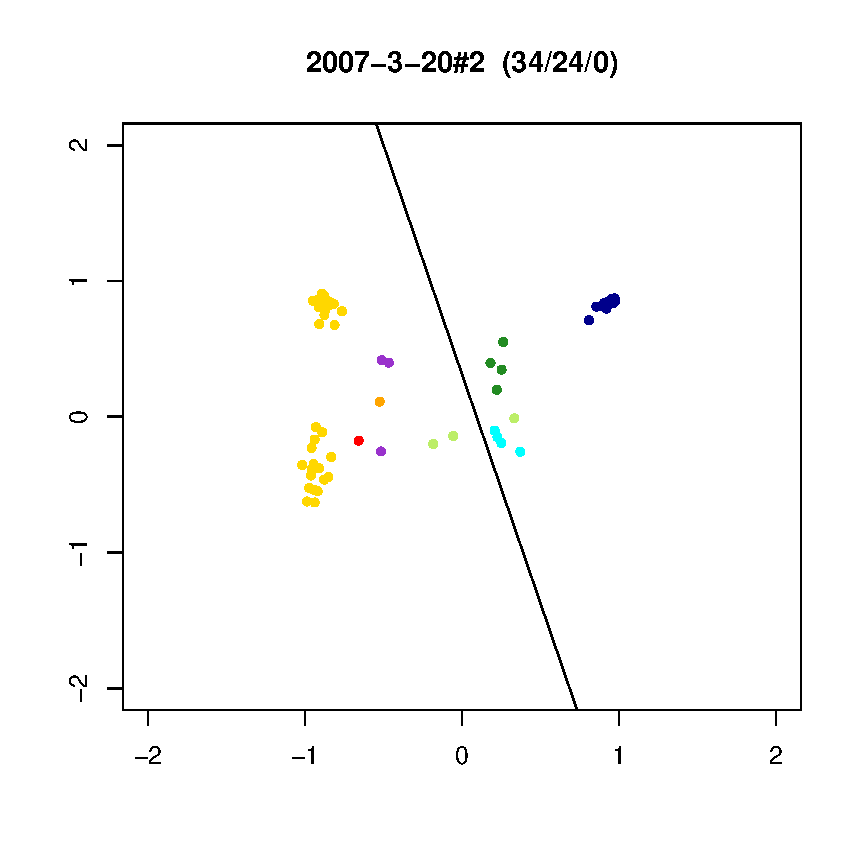
\includegraphics[width=4cm]{cutline25.pdf} &
   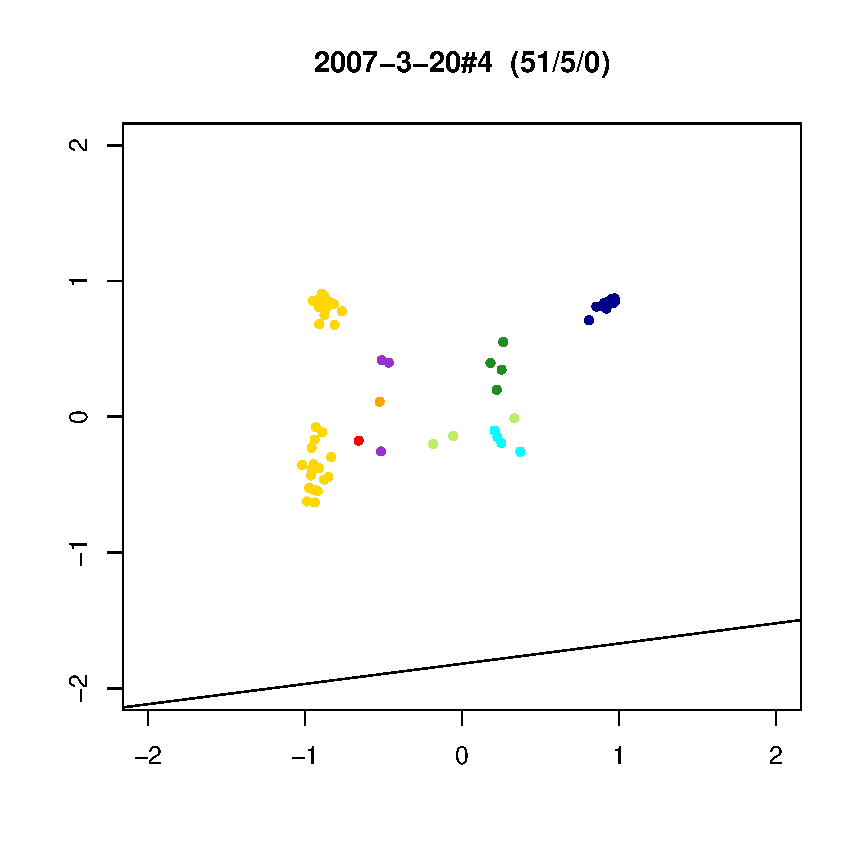
\includegraphics[width=4cm]{cutline26.pdf} &
   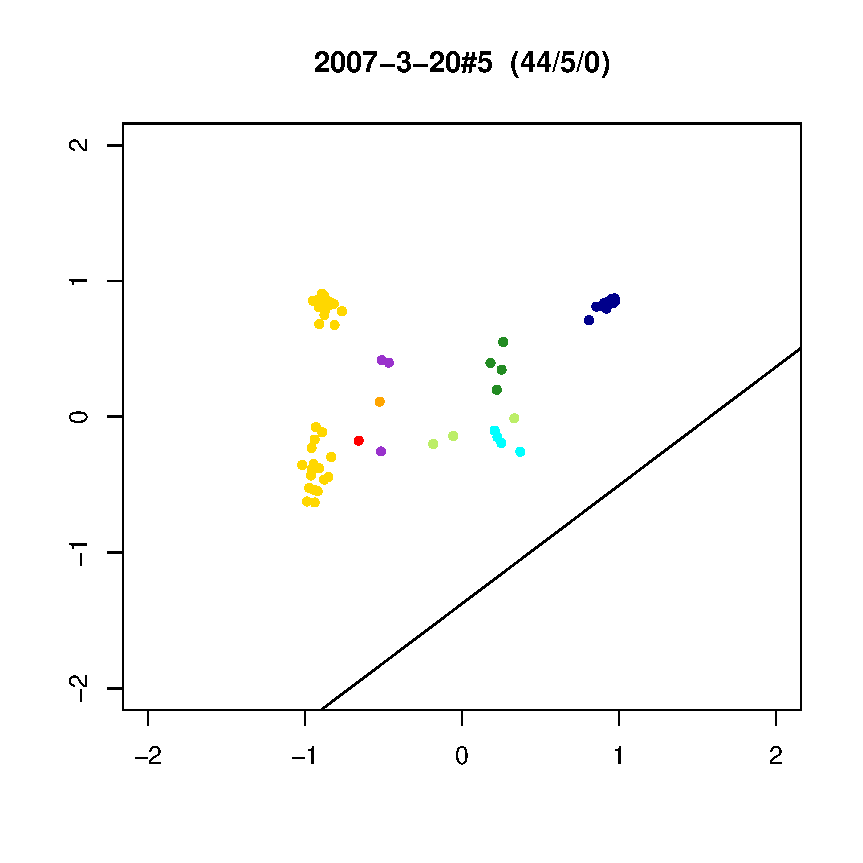
\includegraphics[width=4cm]{cutline27.pdf} &
   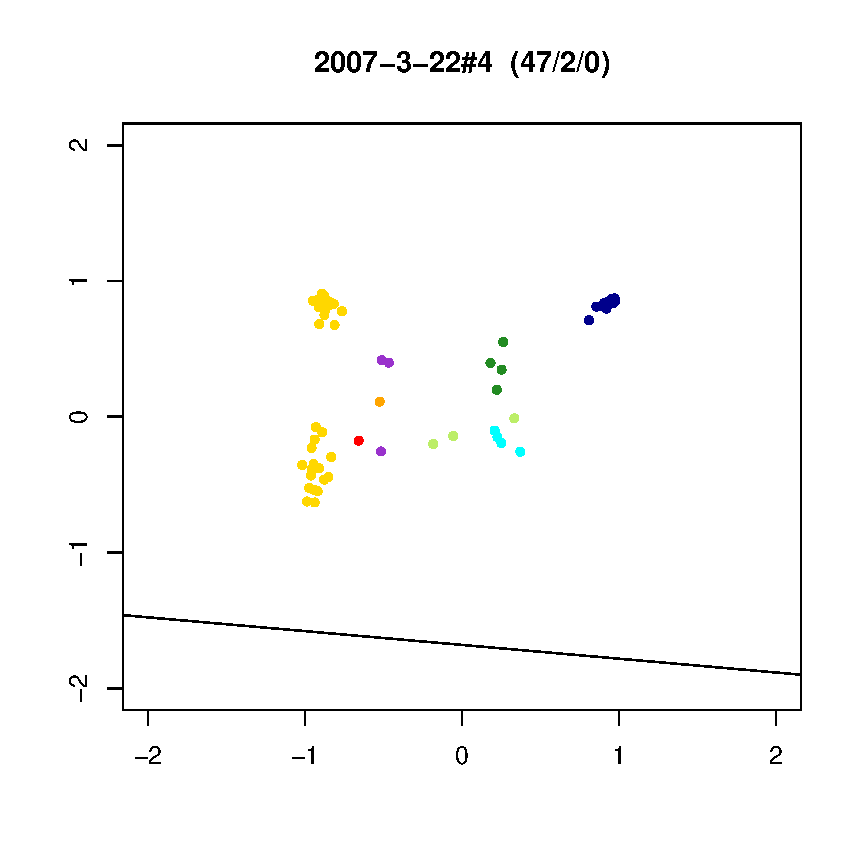
\includegraphics[width=4cm]{cutline28.pdf} \\
   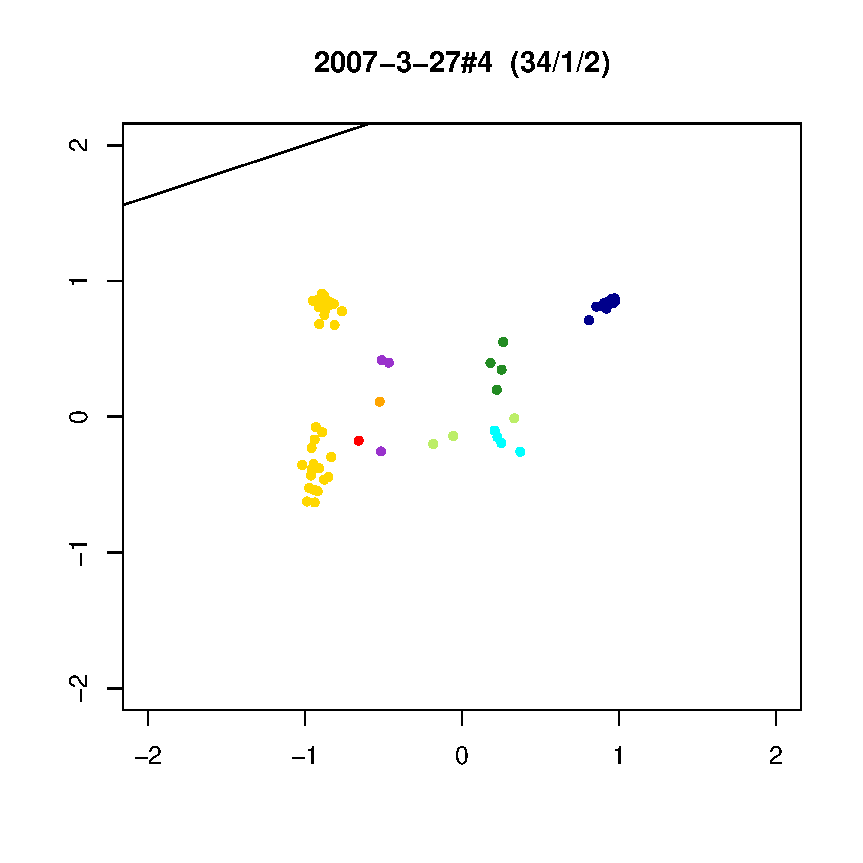
\includegraphics[width=4cm]{cutline29.pdf} &
   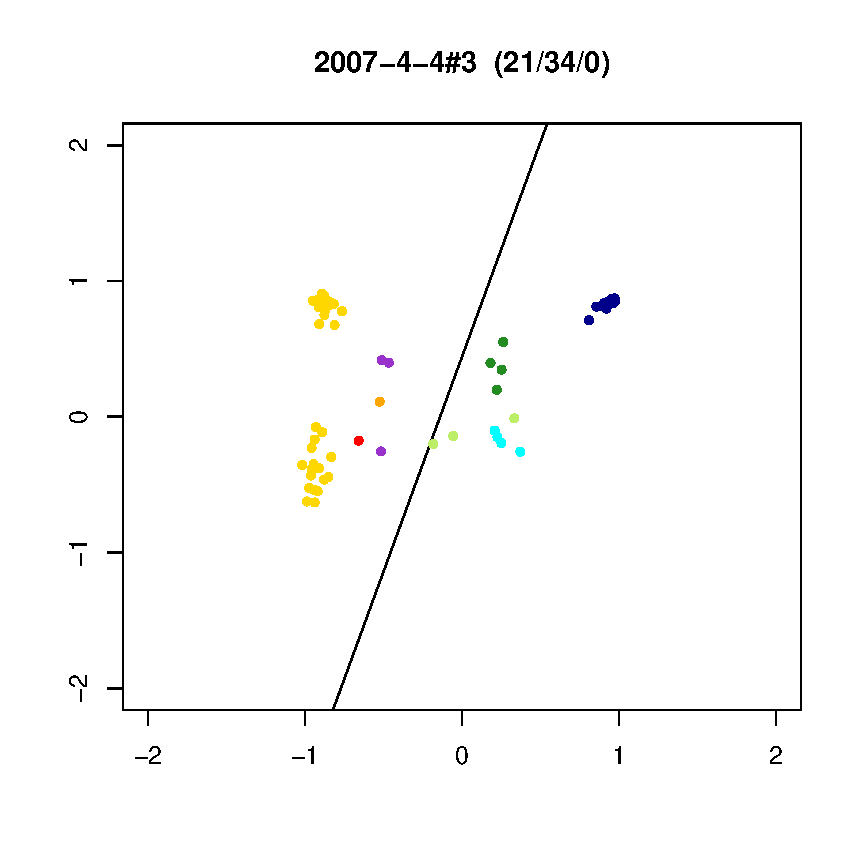
\includegraphics[width=4cm]{cutline30.pdf} &
   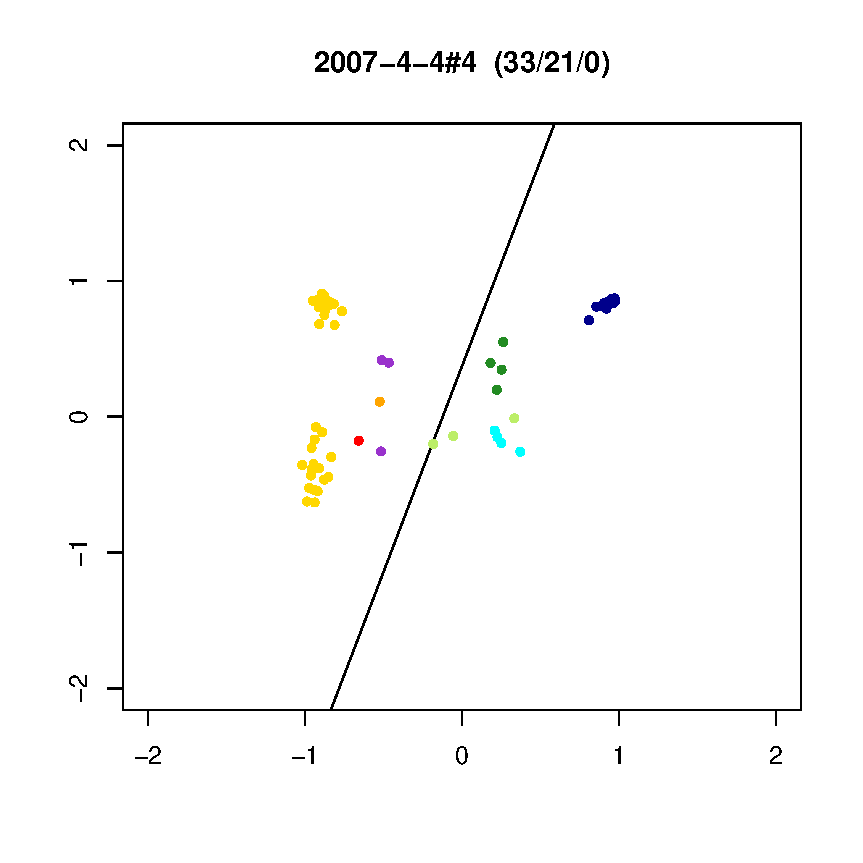
\includegraphics[width=4cm]{cutline31.pdf} &
   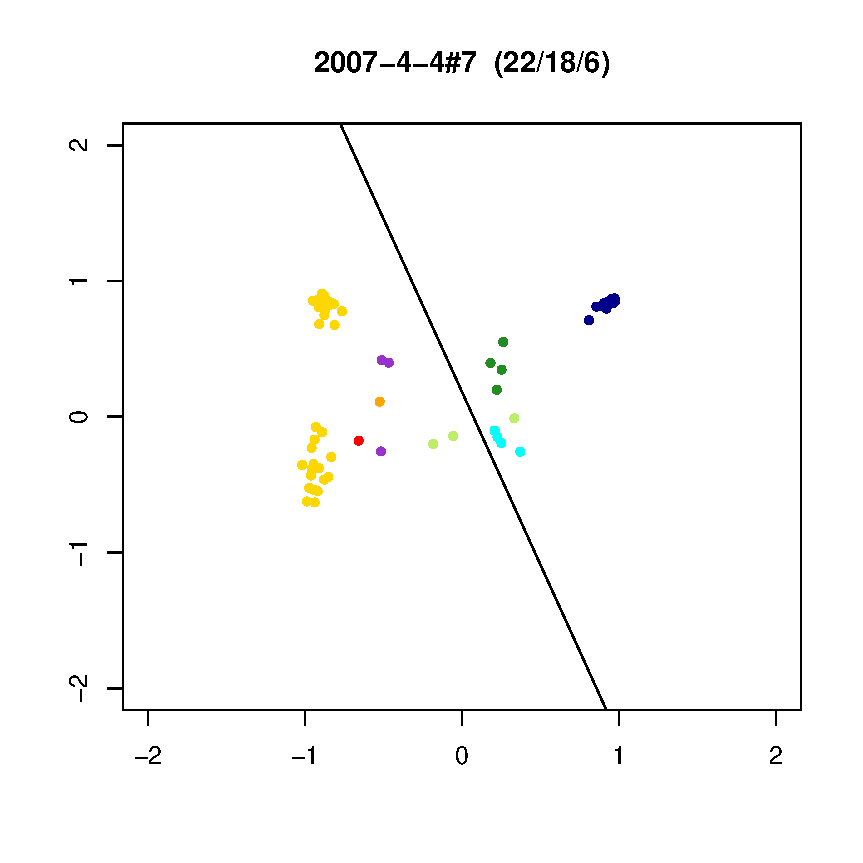
\includegraphics[width=4cm]{cutline32.pdf} \\
   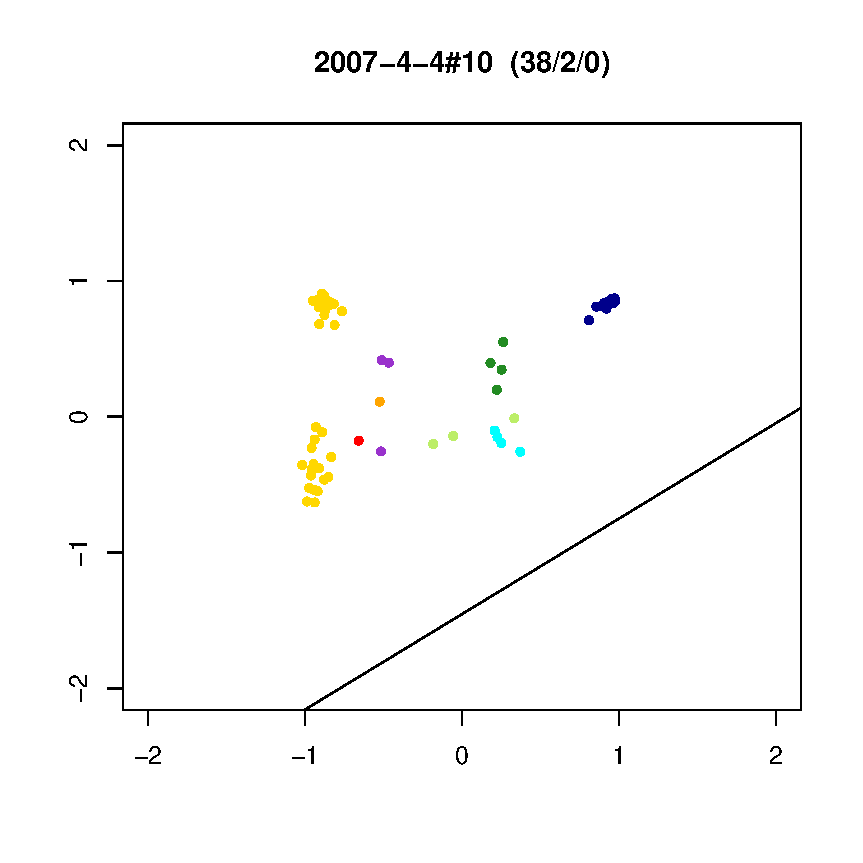
\includegraphics[width=4cm]{cutline33.pdf} &
   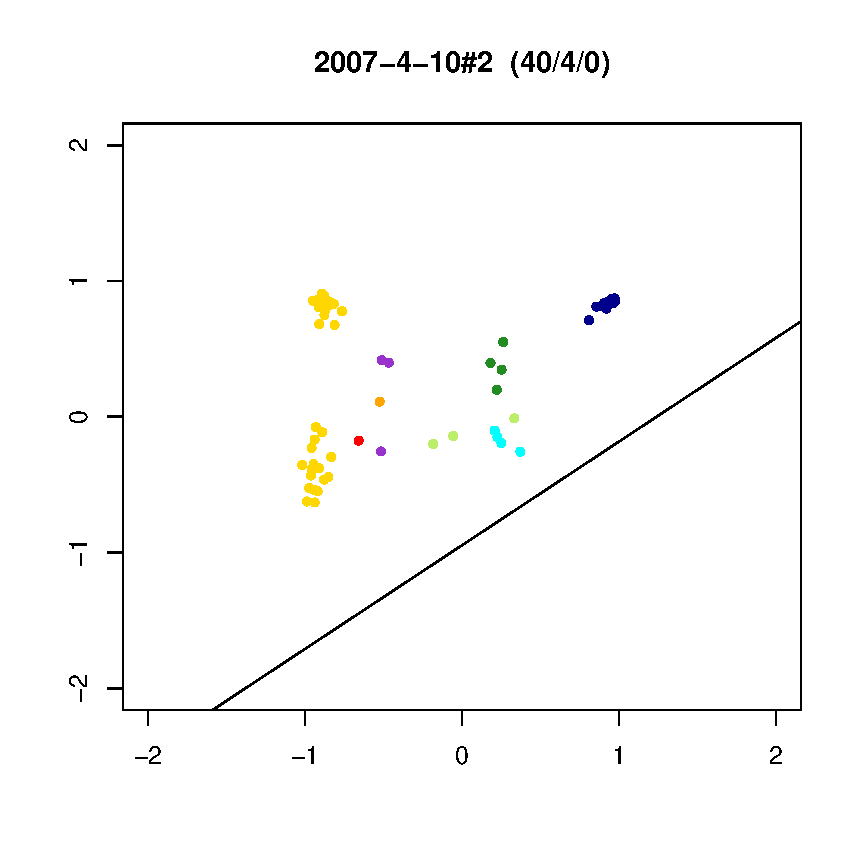
\includegraphics[width=4cm]{cutline34.pdf} &
   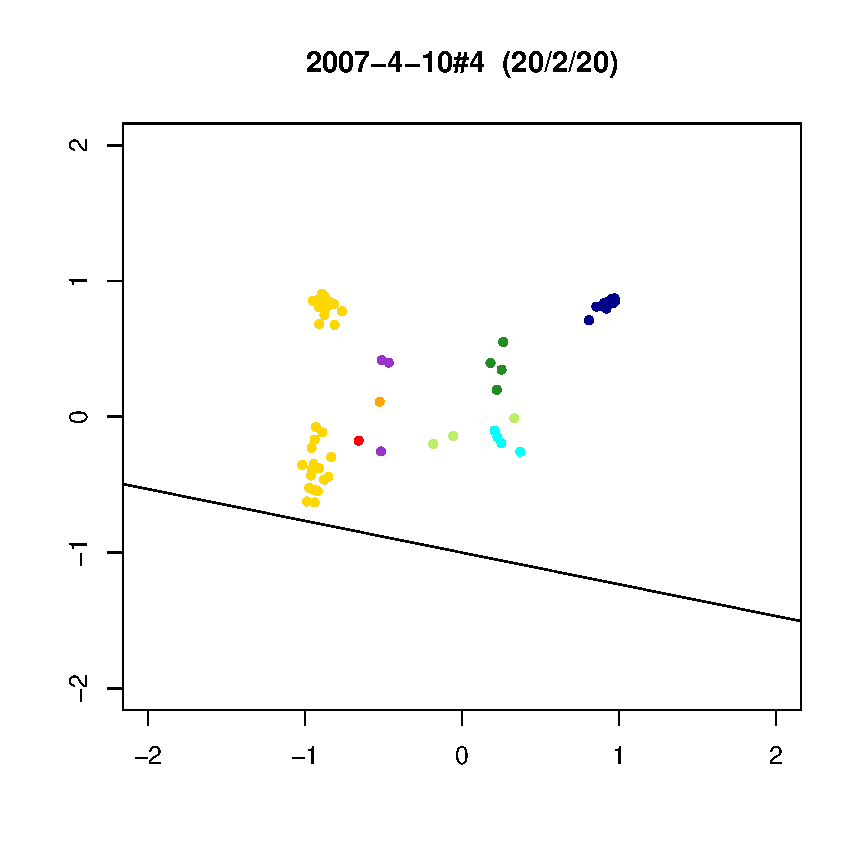
\includegraphics[width=4cm]{cutline35.pdf} &
   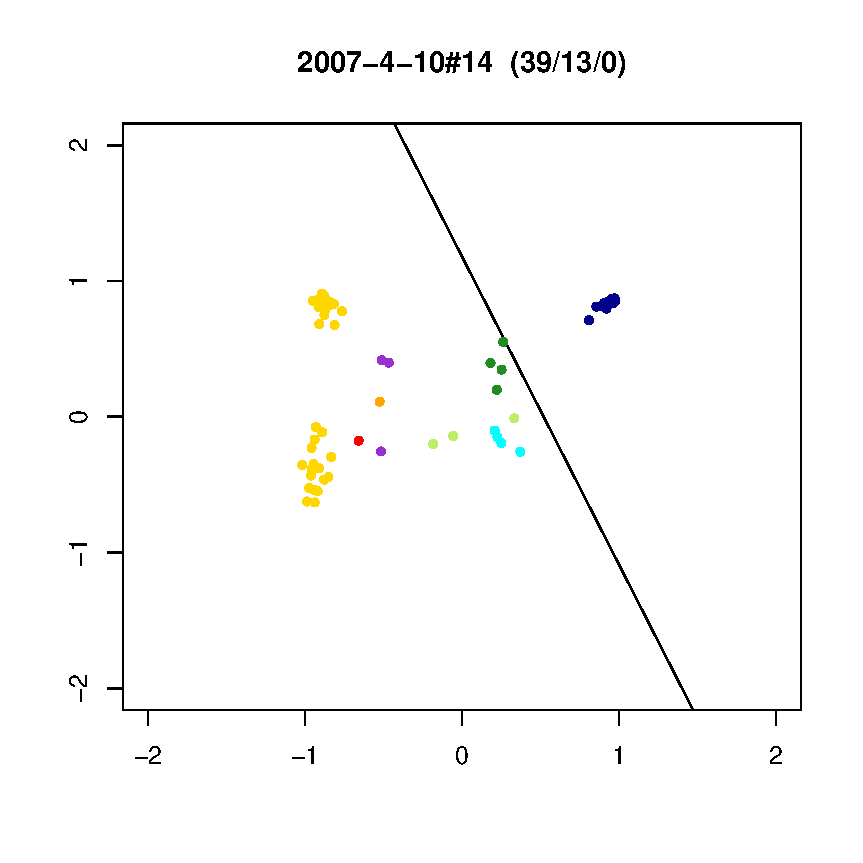
\includegraphics[width=4cm]{cutline36.pdf} \\
   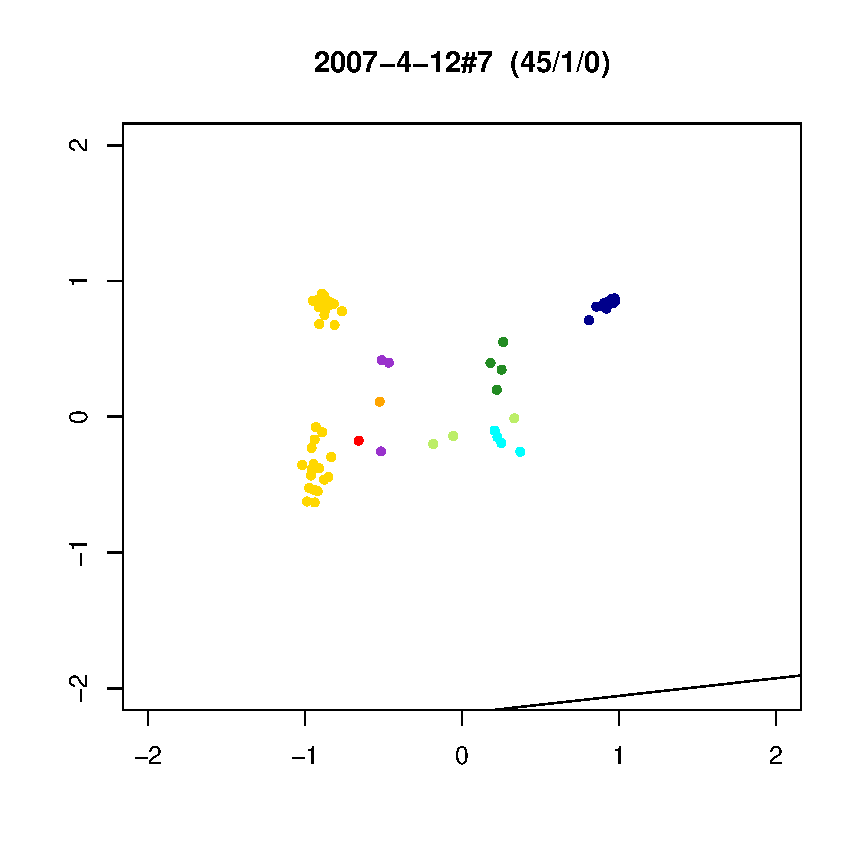
\includegraphics[width=4cm]{cutline37.pdf} &
   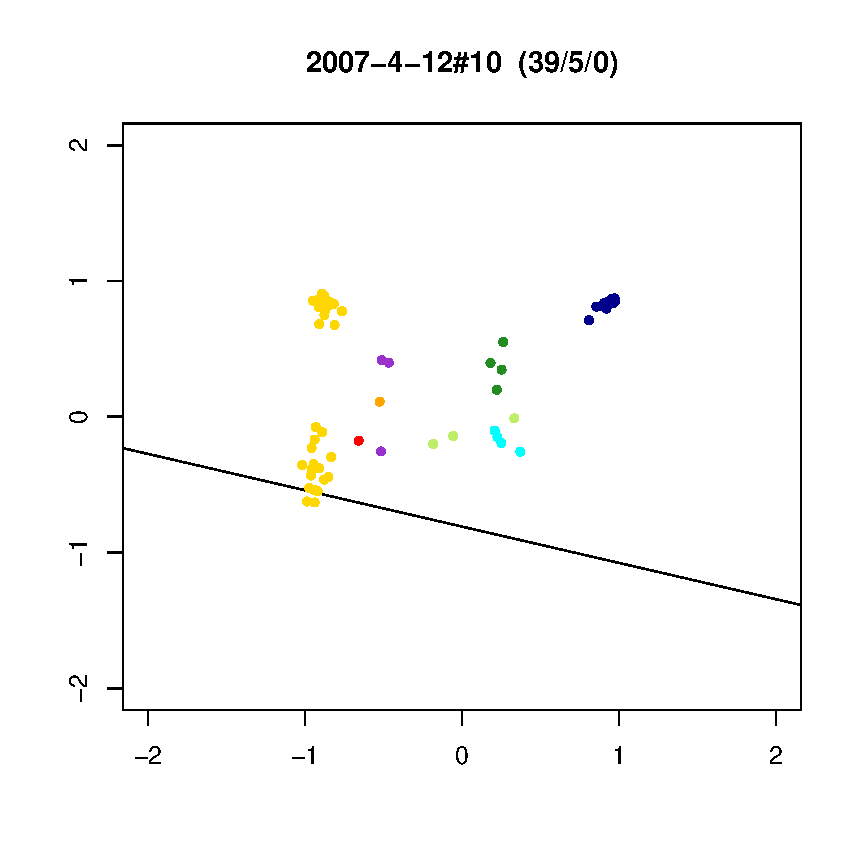
\includegraphics[width=4cm]{cutline38.pdf} &
   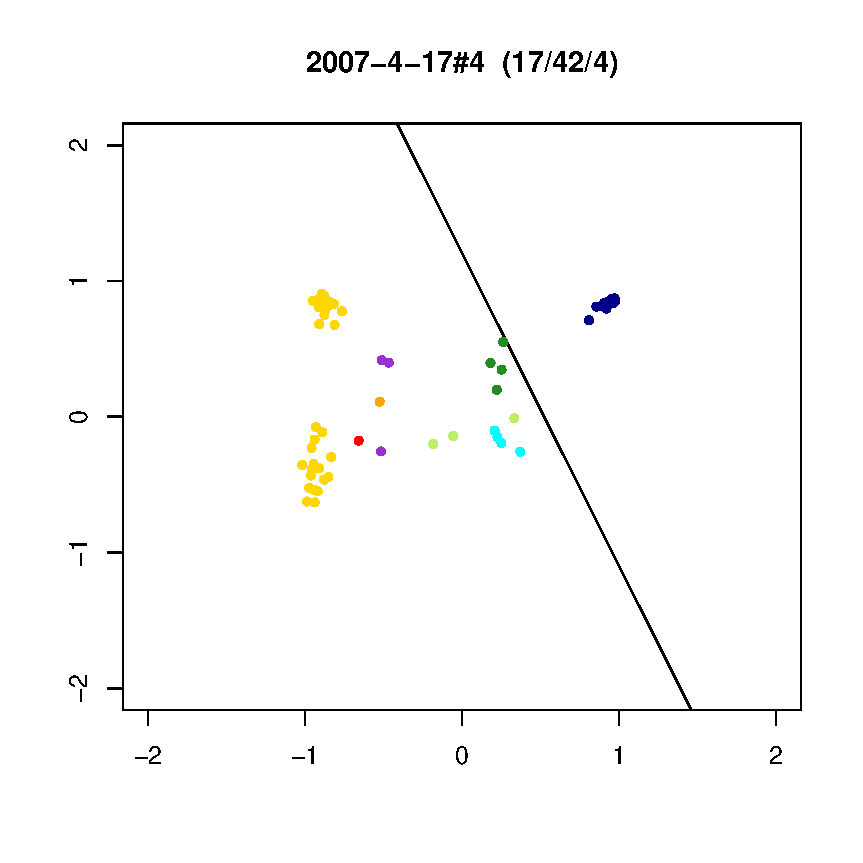
\includegraphics[width=4cm]{cutline39.pdf} &
   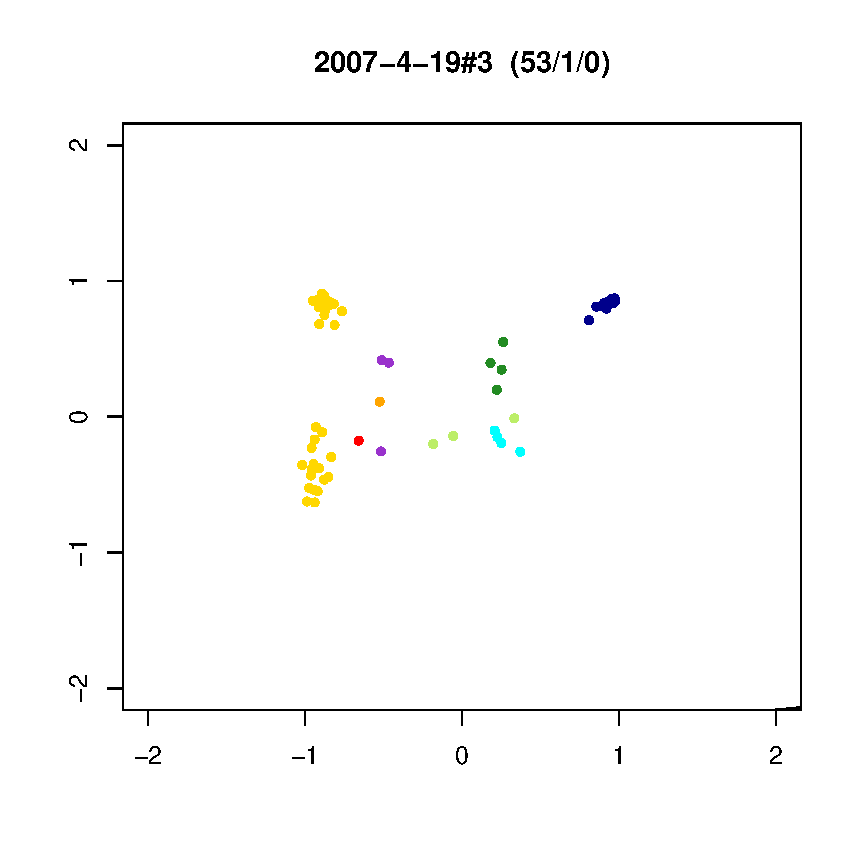
\includegraphics[width=4cm]{cutline40.pdf} \\
\end{tabular}
\end{center}

\newpage

\begin{center}
\begin{tabular}{ccccc}
   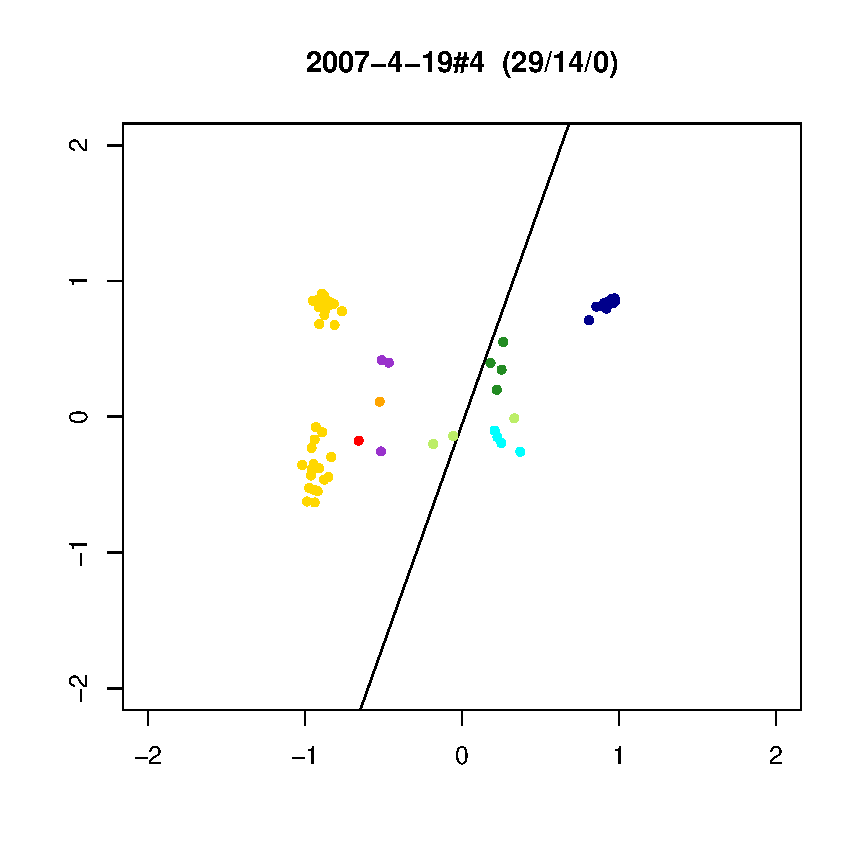
\includegraphics[width=4cm]{cutline41.pdf} &
   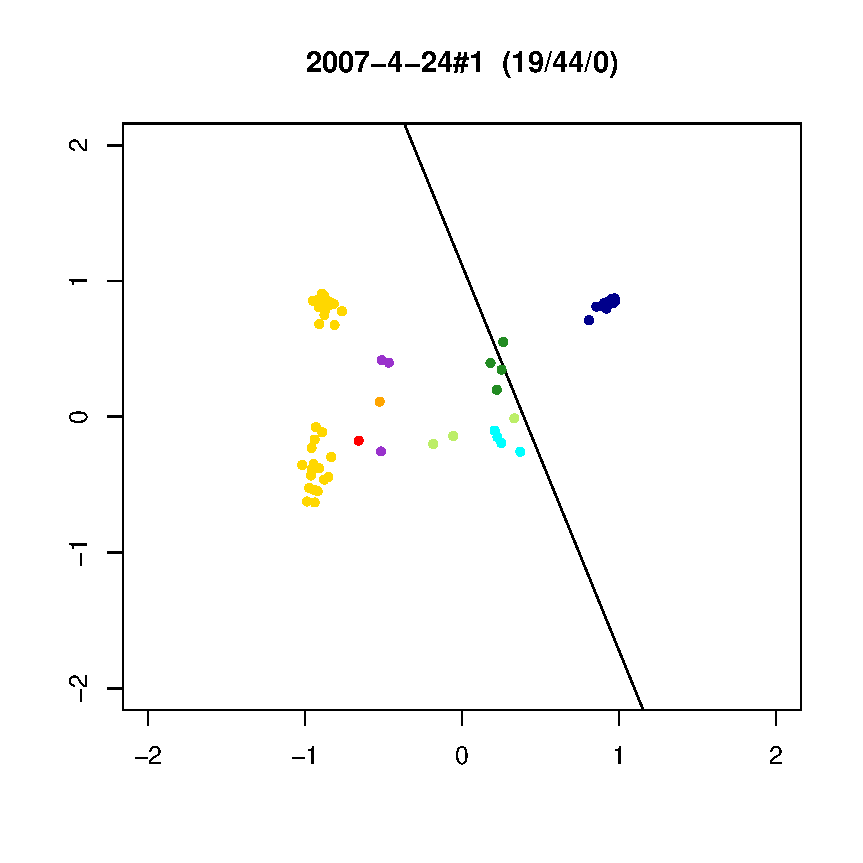
\includegraphics[width=4cm]{cutline42.pdf} &
   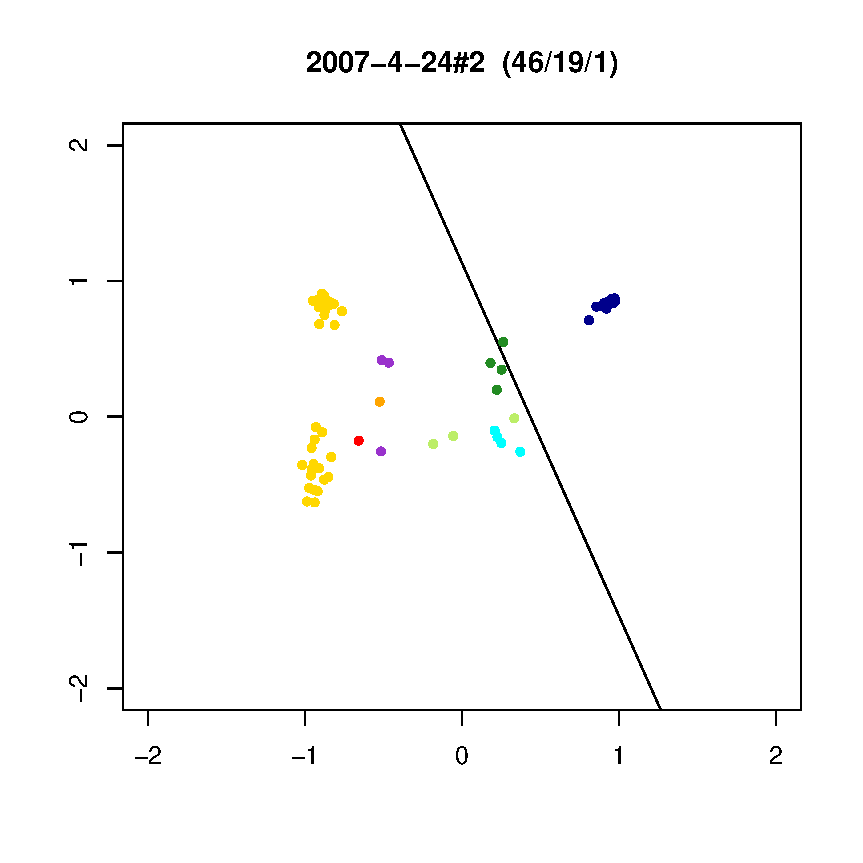
\includegraphics[width=4cm]{cutline43.pdf} &
   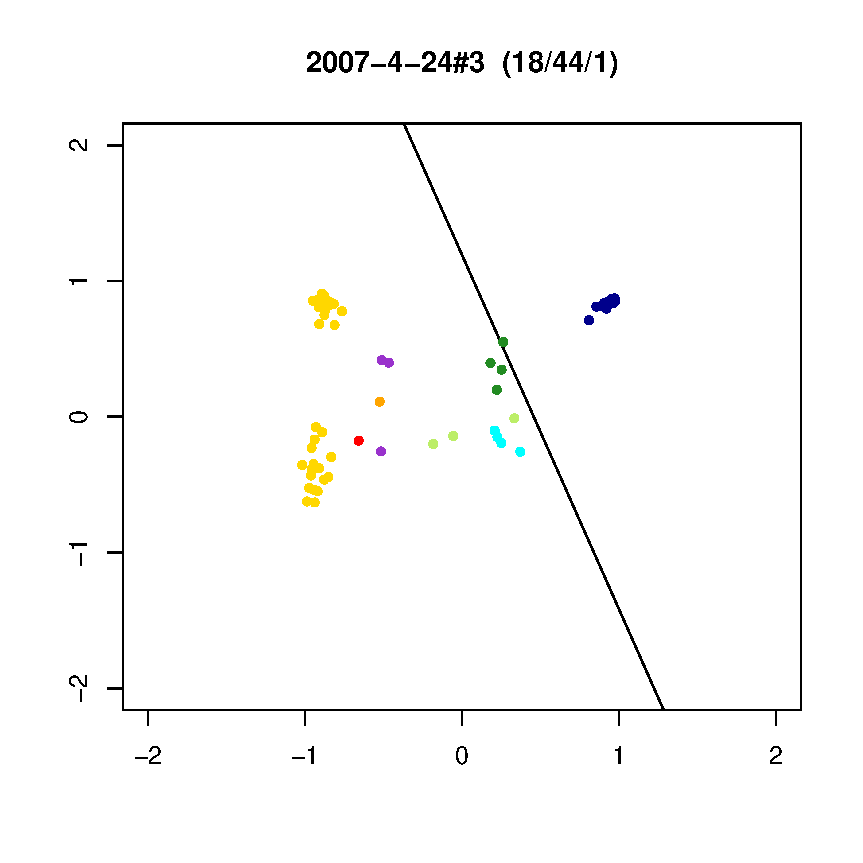
\includegraphics[width=4cm]{cutline44.pdf} \\
   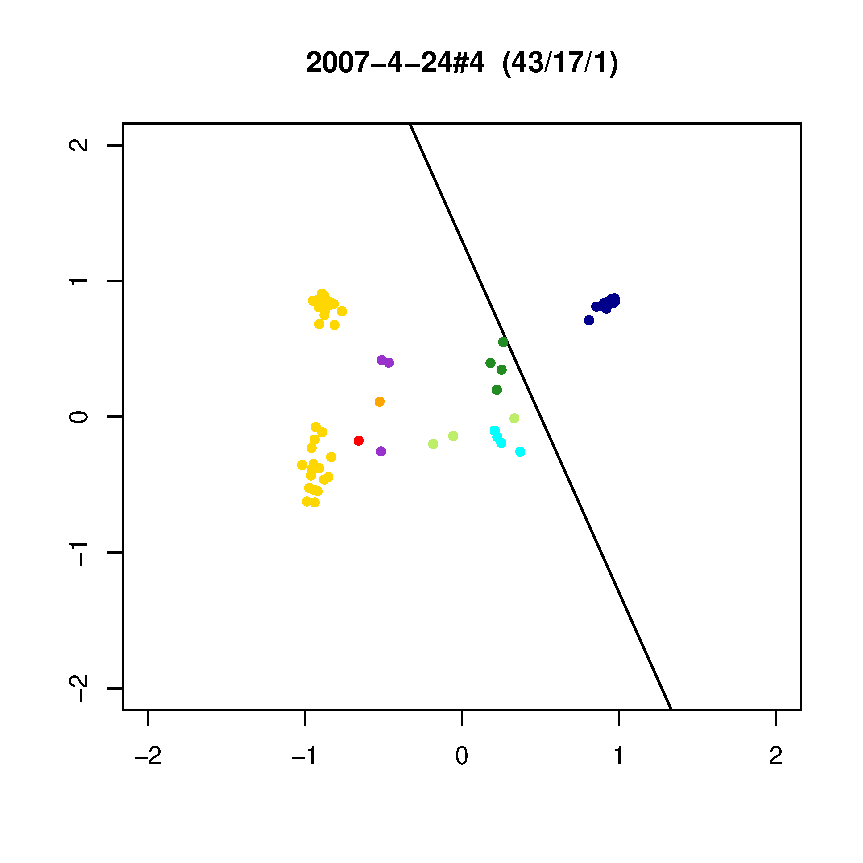
\includegraphics[width=4cm]{cutline45.pdf} &
   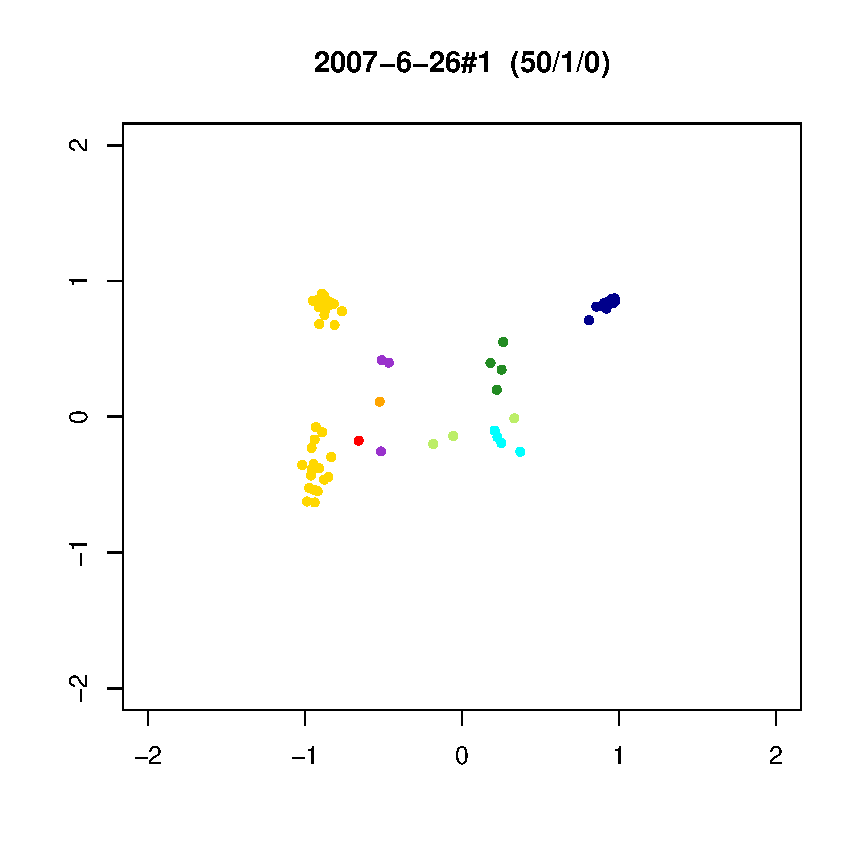
\includegraphics[width=4cm]{cutline46.pdf} &
   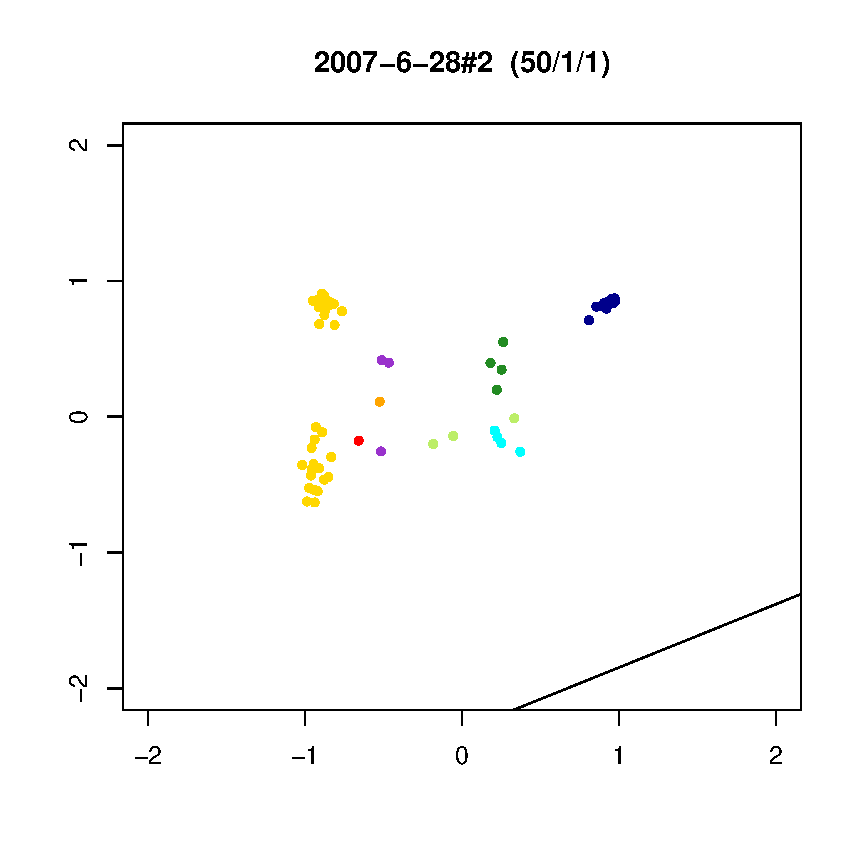
\includegraphics[width=4cm]{cutline47.pdf} &
   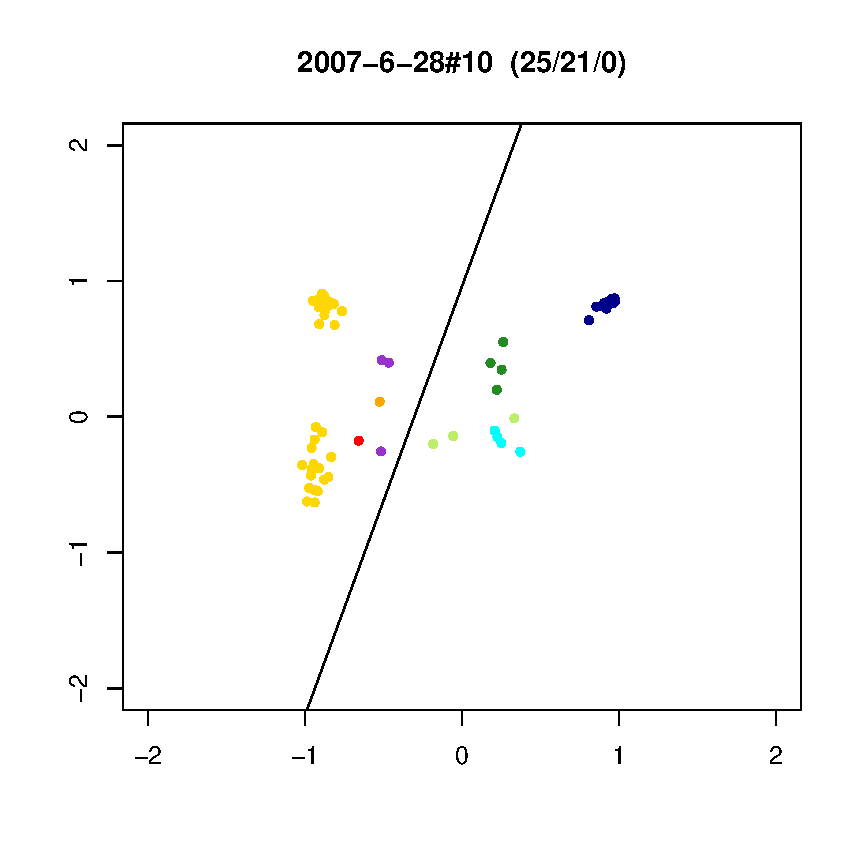
\includegraphics[width=4cm]{cutline48.pdf} \\
   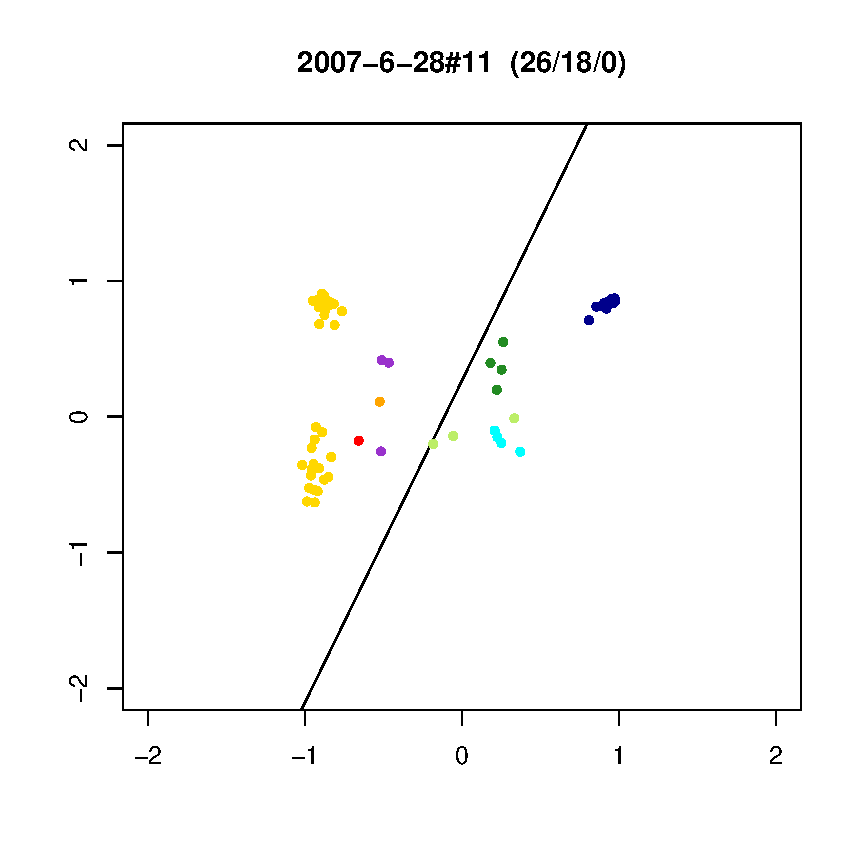
\includegraphics[width=4cm]{cutline49.pdf} &
   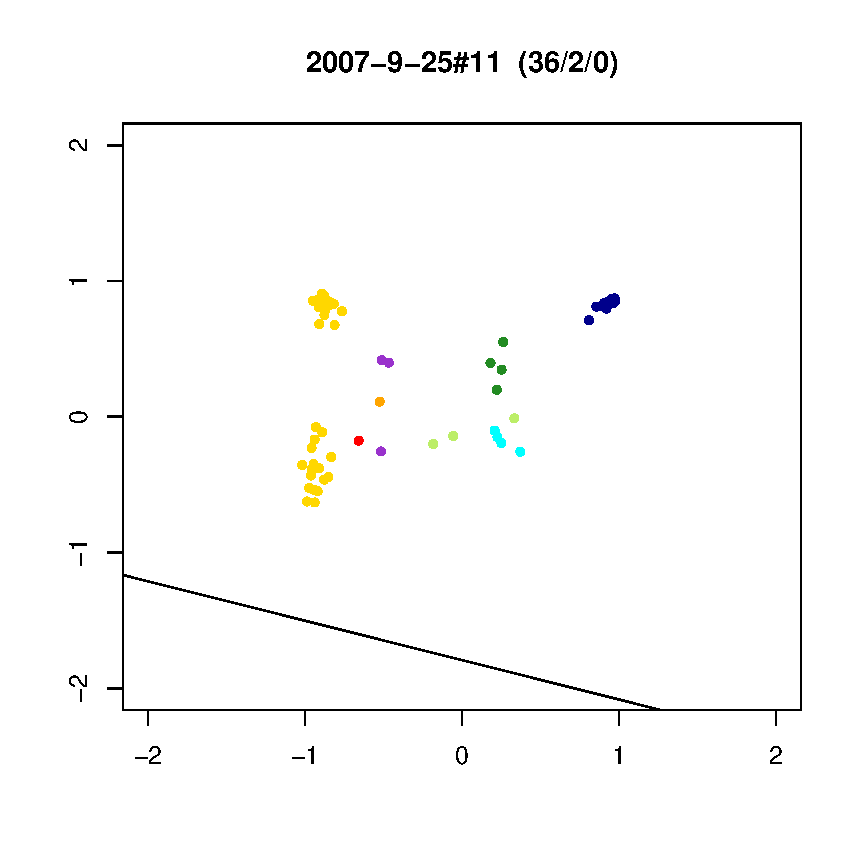
\includegraphics[width=4cm]{cutline50.pdf} &
   \includegraphics[width=4cm]{cutline51.pdf} &
   \includegraphics[width=4cm]{cutline52.pdf} \\
   \includegraphics[width=4cm]{cutline53.pdf} &
   \includegraphics[width=4cm]{cutline54.pdf} &
   \includegraphics[width=4cm]{cutline55.pdf} &
   \includegraphics[width=4cm]{cutline56.pdf} \\
   \includegraphics[width=4cm]{cutline57.pdf} &
   \includegraphics[width=4cm]{cutline58.pdf} &
   \includegraphics[width=4cm]{cutline59.pdf} &
   \includegraphics[width=4cm]{cutline60.pdf} \\
\end{tabular}
\end{center}

\newpage

\begin{center}
\begin{tabular}{ccccc}
   \includegraphics[width=4cm]{cutline61.pdf} &
   \includegraphics[width=4cm]{cutline62.pdf} &
   \includegraphics[width=4cm]{cutline63.pdf} &
   \includegraphics[width=4cm]{cutline64.pdf} \\
   \includegraphics[width=4cm]{cutline65.pdf} &
   \includegraphics[width=4cm]{cutline66.pdf} &
   \includegraphics[width=4cm]{cutline67.pdf} &
   \includegraphics[width=4cm]{cutline68.pdf} \\
   \includegraphics[width=4cm]{cutline69.pdf} &
   \includegraphics[width=4cm]{cutline70.pdf} &
   \includegraphics[width=4cm]{cutline71.pdf} &
   \includegraphics[width=4cm]{cutline72.pdf} \\
   \includegraphics[width=4cm]{cutline73.pdf} &
   \includegraphics[width=4cm]{cutline74.pdf} &
   \includegraphics[width=4cm]{cutline75.pdf} &
   \includegraphics[width=4cm]{cutline76.pdf} \\
   \includegraphics[width=4cm]{cutline77.pdf} &
   \includegraphics[width=4cm]{cutline78.pdf} &
   \includegraphics[width=4cm]{cutline79.pdf} &
   \includegraphics[width=4cm]{cutline80.pdf} \\
\end{tabular}
\end{center}

\newpage

\begin{center}
\begin{tabular}{ccccc}
   \includegraphics[width=4cm]{cutline81.pdf} &
   \includegraphics[width=4cm]{cutline82.pdf} &
   \includegraphics[width=4cm]{cutline83.pdf} &
   \includegraphics[width=4cm]{cutline84.pdf} \\
   \includegraphics[width=4cm]{cutline85.pdf} &
   \includegraphics[width=4cm]{cutline86.pdf} &
   \includegraphics[width=4cm]{cutline87.pdf} &
   \includegraphics[width=4cm]{cutline88.pdf} \\
   \includegraphics[width=4cm]{cutline89.pdf} &
   \includegraphics[width=4cm]{cutline90.pdf} &
   \includegraphics[width=4cm]{cutline91.pdf} &
   \includegraphics[width=4cm]{cutline92.pdf} \\
   \includegraphics[width=4cm]{cutline93.pdf} &
   \includegraphics[width=4cm]{cutline94.pdf} &
   \includegraphics[width=4cm]{cutline95.pdf} &
   \includegraphics[width=4cm]{cutline96.pdf} \\
   \includegraphics[width=4cm]{cutline97.pdf} &
   \includegraphics[width=4cm]{cutline98.pdf} &
   \includegraphics[width=4cm]{cutline99.pdf} &
   \includegraphics[width=4cm]{cutline100.pdf} \\
\end{tabular}
\end{center}

\newpage

\begin{center}
\begin{tabular}{ccccc}
   \includegraphics[width=4cm]{cutline101.pdf} &
   \includegraphics[width=4cm]{cutline102.pdf} &
   \includegraphics[width=4cm]{cutline103.pdf} &
   \includegraphics[width=4cm]{cutline104.pdf} \\
   \includegraphics[width=4cm]{cutline105.pdf} &
   \includegraphics[width=4cm]{cutline106.pdf} &
   \includegraphics[width=4cm]{cutline107.pdf} &
   \includegraphics[width=4cm]{cutline108.pdf} \\
   \includegraphics[width=4cm]{cutline109.pdf} &
   \includegraphics[width=4cm]{cutline110.pdf} &
   \includegraphics[width=4cm]{cutline111.pdf} &
   \includegraphics[width=4cm]{cutline112.pdf} \\
   \includegraphics[width=4cm]{cutline113.pdf} &
   \includegraphics[width=4cm]{cutline114.pdf} &
   \includegraphics[width=4cm]{cutline115.pdf} &
   \includegraphics[width=4cm]{cutline116.pdf} \\
   \includegraphics[width=4cm]{cutline117.pdf} &
   \includegraphics[width=4cm]{cutline118.pdf} &
   \includegraphics[width=4cm]{cutline119.pdf} &
   \includegraphics[width=4cm]{cutline120.pdf} \\
\end{tabular}
\end{center}

\newpage

\begin{center}
\begin{tabular}{ccccc}
   \includegraphics[width=4cm]{cutline121.pdf} &
   \includegraphics[width=4cm]{cutline122.pdf} &
   \includegraphics[width=4cm]{cutline123.pdf} &
   \includegraphics[width=4cm]{cutline124.pdf} \\
   \includegraphics[width=4cm]{cutline125.pdf} &
   \includegraphics[width=4cm]{cutline126.pdf} &
   \includegraphics[width=4cm]{cutline127.pdf} &
   \includegraphics[width=4cm]{cutline128.pdf} \\
   \includegraphics[width=4cm]{cutline129.pdf} &
   \includegraphics[width=4cm]{cutline130.pdf} &
   \includegraphics[width=4cm]{cutline131.pdf} &
   \includegraphics[width=4cm]{cutline132.pdf} \\
   \includegraphics[width=4cm]{cutline133.pdf} &
   \includegraphics[width=4cm]{cutline134.pdf} &
   \includegraphics[width=4cm]{cutline135.pdf} &
   \includegraphics[width=4cm]{cutline136.pdf} \\
   \includegraphics[width=4cm]{cutline137.pdf} &
   \includegraphics[width=4cm]{cutline138.pdf} &
   \includegraphics[width=4cm]{cutline139.pdf} &
   \includegraphics[width=4cm]{cutline140.pdf} \\
\end{tabular}
\end{center}

\newpage

\begin{center}
\begin{tabular}{ccccc}
   \includegraphics[width=4cm]{cutline141.pdf} &
   \includegraphics[width=4cm]{cutline142.pdf} &
   \includegraphics[width=4cm]{cutline143.pdf} &
   \includegraphics[width=4cm]{cutline144.pdf} \\
   \includegraphics[width=4cm]{cutline145.pdf} &
   \includegraphics[width=4cm]{cutline146.pdf} &
   \includegraphics[width=4cm]{cutline147.pdf} &
   \includegraphics[width=4cm]{cutline148.pdf} \\
   \includegraphics[width=4cm]{cutline149.pdf} &
   \includegraphics[width=4cm]{cutline150.pdf} &
   \includegraphics[width=4cm]{cutline151.pdf} &
   \includegraphics[width=4cm]{cutline152.pdf} \\
   \includegraphics[width=4cm]{cutline153.pdf} &
   \includegraphics[width=4cm]{cutline154.pdf} &
   \includegraphics[width=4cm]{cutline155.pdf} &
   \includegraphics[width=4cm]{cutline156.pdf} \\
   \includegraphics[width=4cm]{cutline157.pdf} &
   \includegraphics[width=4cm]{cutline158.pdf} &
   \includegraphics[width=4cm]{cutline159.pdf} &
   \includegraphics[width=4cm]{cutline160.pdf} \\
\end{tabular}
\end{center}

\newpage

\begin{center}
\begin{tabular}{ccccc}
   \includegraphics[width=4cm]{cutline161.pdf} &
   \includegraphics[width=4cm]{cutline162.pdf} &
   \includegraphics[width=4cm]{cutline163.pdf} &
   \includegraphics[width=4cm]{cutline164.pdf} \\
   \includegraphics[width=4cm]{cutline165.pdf} &
   \includegraphics[width=4cm]{cutline166.pdf} &
   \includegraphics[width=4cm]{cutline167.pdf} &
   \includegraphics[width=4cm]{cutline168.pdf} \\
   \includegraphics[width=4cm]{cutline169.pdf} &
   \includegraphics[width=4cm]{cutline170.pdf} &
   \includegraphics[width=4cm]{cutline171.pdf} &
   \includegraphics[width=4cm]{cutline172.pdf} \\
   \includegraphics[width=4cm]{cutline173.pdf} &
   \includegraphics[width=4cm]{cutline174.pdf} &
   \includegraphics[width=4cm]{cutline175.pdf} &
   \includegraphics[width=4cm]{cutline176.pdf} \\
\end{tabular}
\end{center}

\end{document}
